% !TEX root = trkjet.tex

The centrality dependence of \RDptr\ for two charged-particle \pt\ intervals: 1.0 -- 1.6~\GeV\ and \mbox{6.3 -- 10.0~\GeV}, and two different \ptjet\ ranges: 126 -- 158 GeV and 200 -- 251 GeV, is presented in Figure~\ref{fig:centdep}. The magnitude of these modifications decreases for more peripheral collisions and \RDptr\ approaches unity in 60 -- 80\% central collisions for both \pt\ ranges, across the entire $ r < 0.8$ range under investigation. 


\begin{figure}[h]
\centerline{
         \begin{tabular}{cc}
            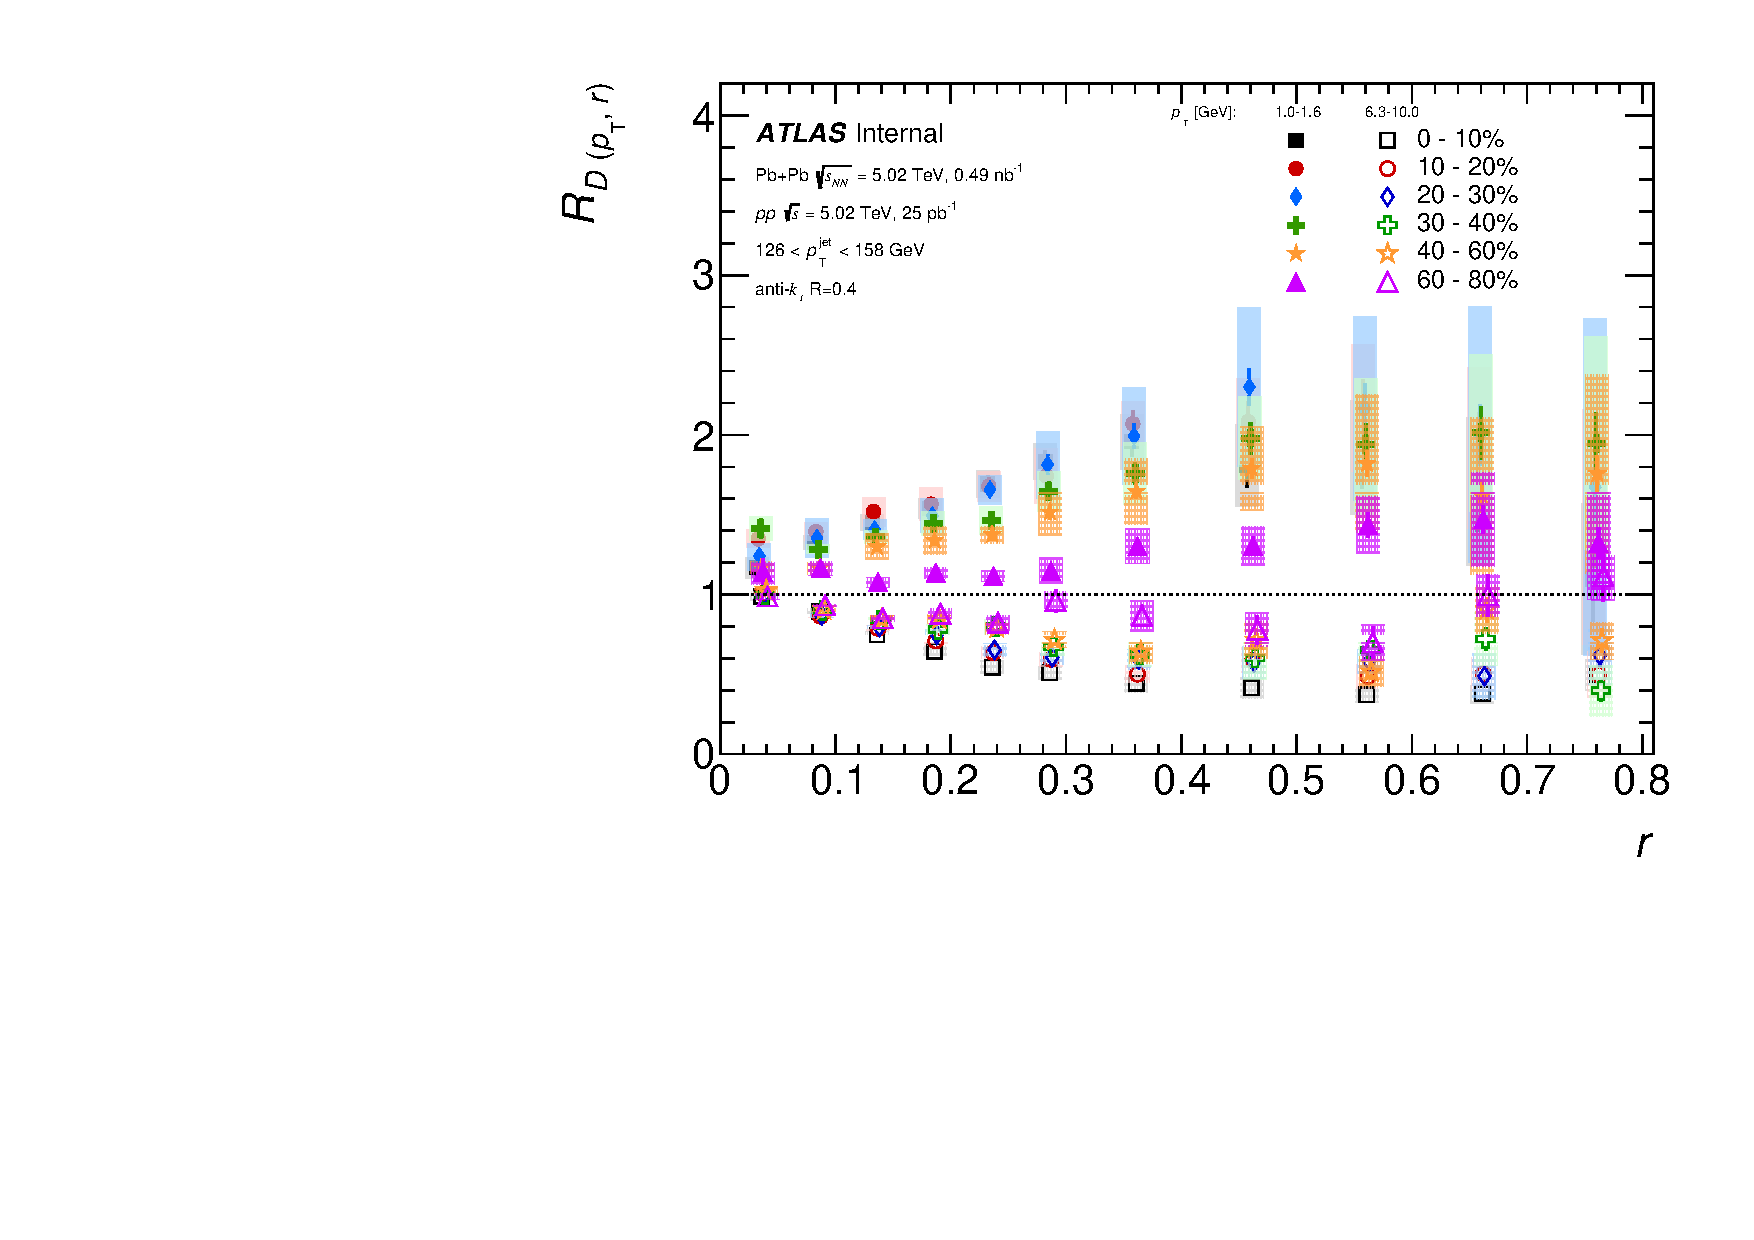
\includegraphics[width=0.5\textwidth]{figures/results/RDpT_final_dR_CONF_data_cent_trk2_6_jet7.pdf} & 
            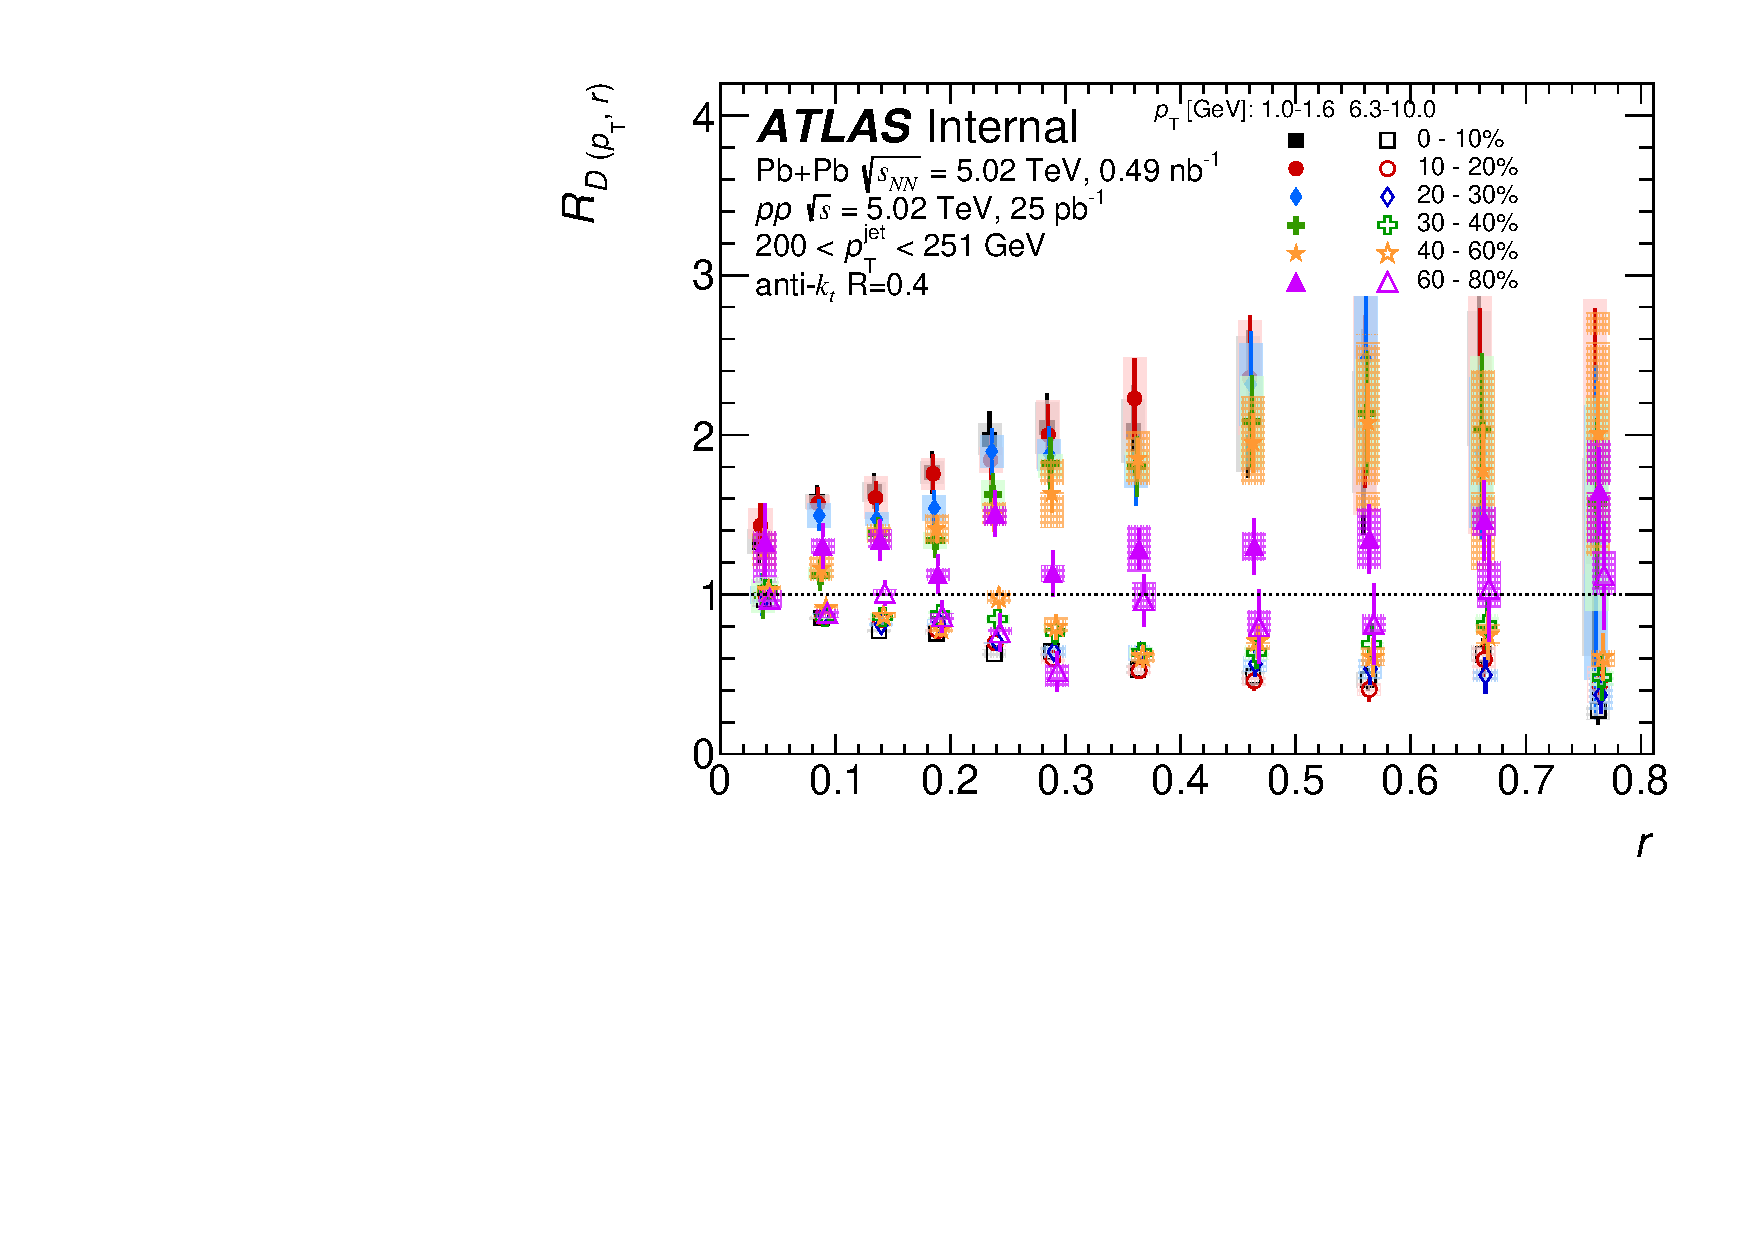
\includegraphics[width=0.5\textwidth]{figures/results/RDpT_final_dR_CONF_data_cent_trk2_6_jet9.pdf} \\
      \end{tabular}
      }
\caption{Ratios of \Dptr\ distributions for \ptjet\ of 126 to 158~\GeV\ (left) and of 200 to 251~\GeV\ (right) in \PbPb\ collisions to \pp\ collisions as a function of angular distance $r$ for two \pt\ selections and six centrality intervals (\pt\ selections are shown by closed and open symbols). The vertical bars on the data points indicate statistical uncertainties while the shaded boxes indicate systematic uncertainties. There are no uncertainties on the \rvar\ values, the finite widths of the shaded boxes are purely aesthetic.}
\label{fig:centdep}
\end{figure}


The \ptjet\ dependence of \RDptr\ for two \pt intervals: 1.0 -- 1.6~\GeV\ and \mbox{6.3 -- 10.0~\GeV}, in 0 -- 10\% central \pbpb\ collisions is presented in Figure~\ref{fig:ptjetdep}. A statistically significant trend of increasing \RDptr\ with increasing \ptjet\ is observed for $0.1 < r < 0.25$ for low pt particles. The higher-\pt\ charged particles have \RDptr\ values that decrease with increasing \rvar; no significant dependence on \ptjet\ is observed. 

\begin{figure}[ht]
\centerline{
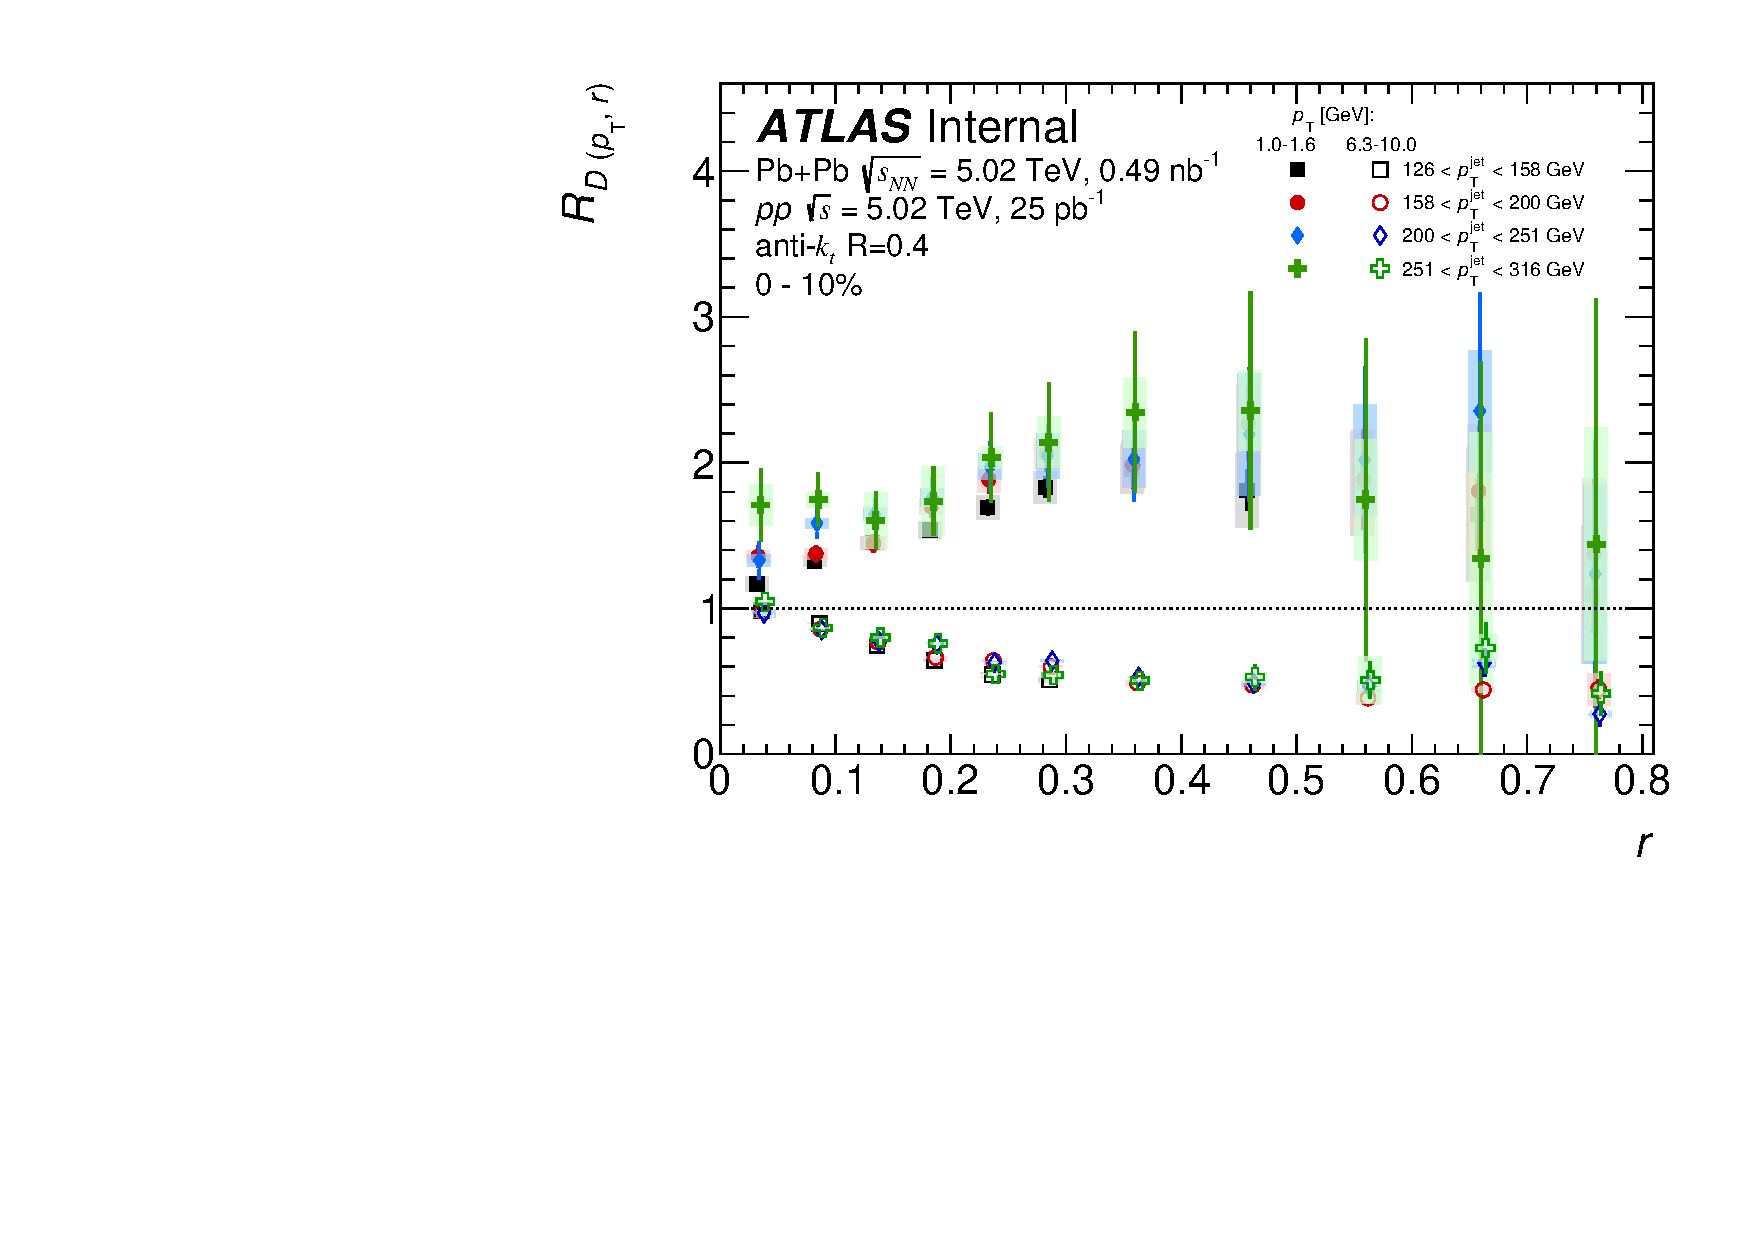
\includegraphics[width=0.8\textwidth]{figures/results/RDpT_final_ratio_dR_CONF_data_trk2_6_cent0.pdf} 
}
\caption{\RDptr\ as a function of \rvar\ for 0--10\% collisions for charged particles with 1.6~$< \pt <$~2.5~\GeV\
(closed symbols) and 6.3~$< \pt <$10.0~\GeV\ (open symbols) for four \ptjet\ selections: 126--158~\GeV, 158--200~\GeV,
200--251~\GeV, and 251--316~\GeV. There are no uncertainties on the \rvar\ values, the finite widths of the shaded boxes are purely aesthetic.}
\label{fig:ptjetdep}
\end{figure}



Differences between the \Dptr\ distributions in \pbpb\ and \pp\ are presented as a function of $r$ for different \pt\ selections in 0 -- 10\% central collisions in Figure~\ref{fig:deltadptr}. 
These distributions indicate an excess (depletion) in the charged-particle yield for \pbpb\ collisions compared to \pp\ collisions for charged particles with low (high) \pt\. This excess ranges from 0.5 to 4 particles at 1 \GeV\ while the depletion is at most 0.5 particles at 10 \GeV. The excess is observed to increase with increasing \ptjet\ for low \pt\ particles.


These observations are in agreement with the previous measurement of jet fragmentation functions \cite{Chatrchyan:2014ava, Sirunyan:2018jqr, Aaboud:2017bzv, PhysRevC.98.024908} and may indicate the dependence of the response of the hot dense matter to the momentum of a jet passing through it. 

\begin{figure}
\centering{
\begin{tabular}{cc}
	 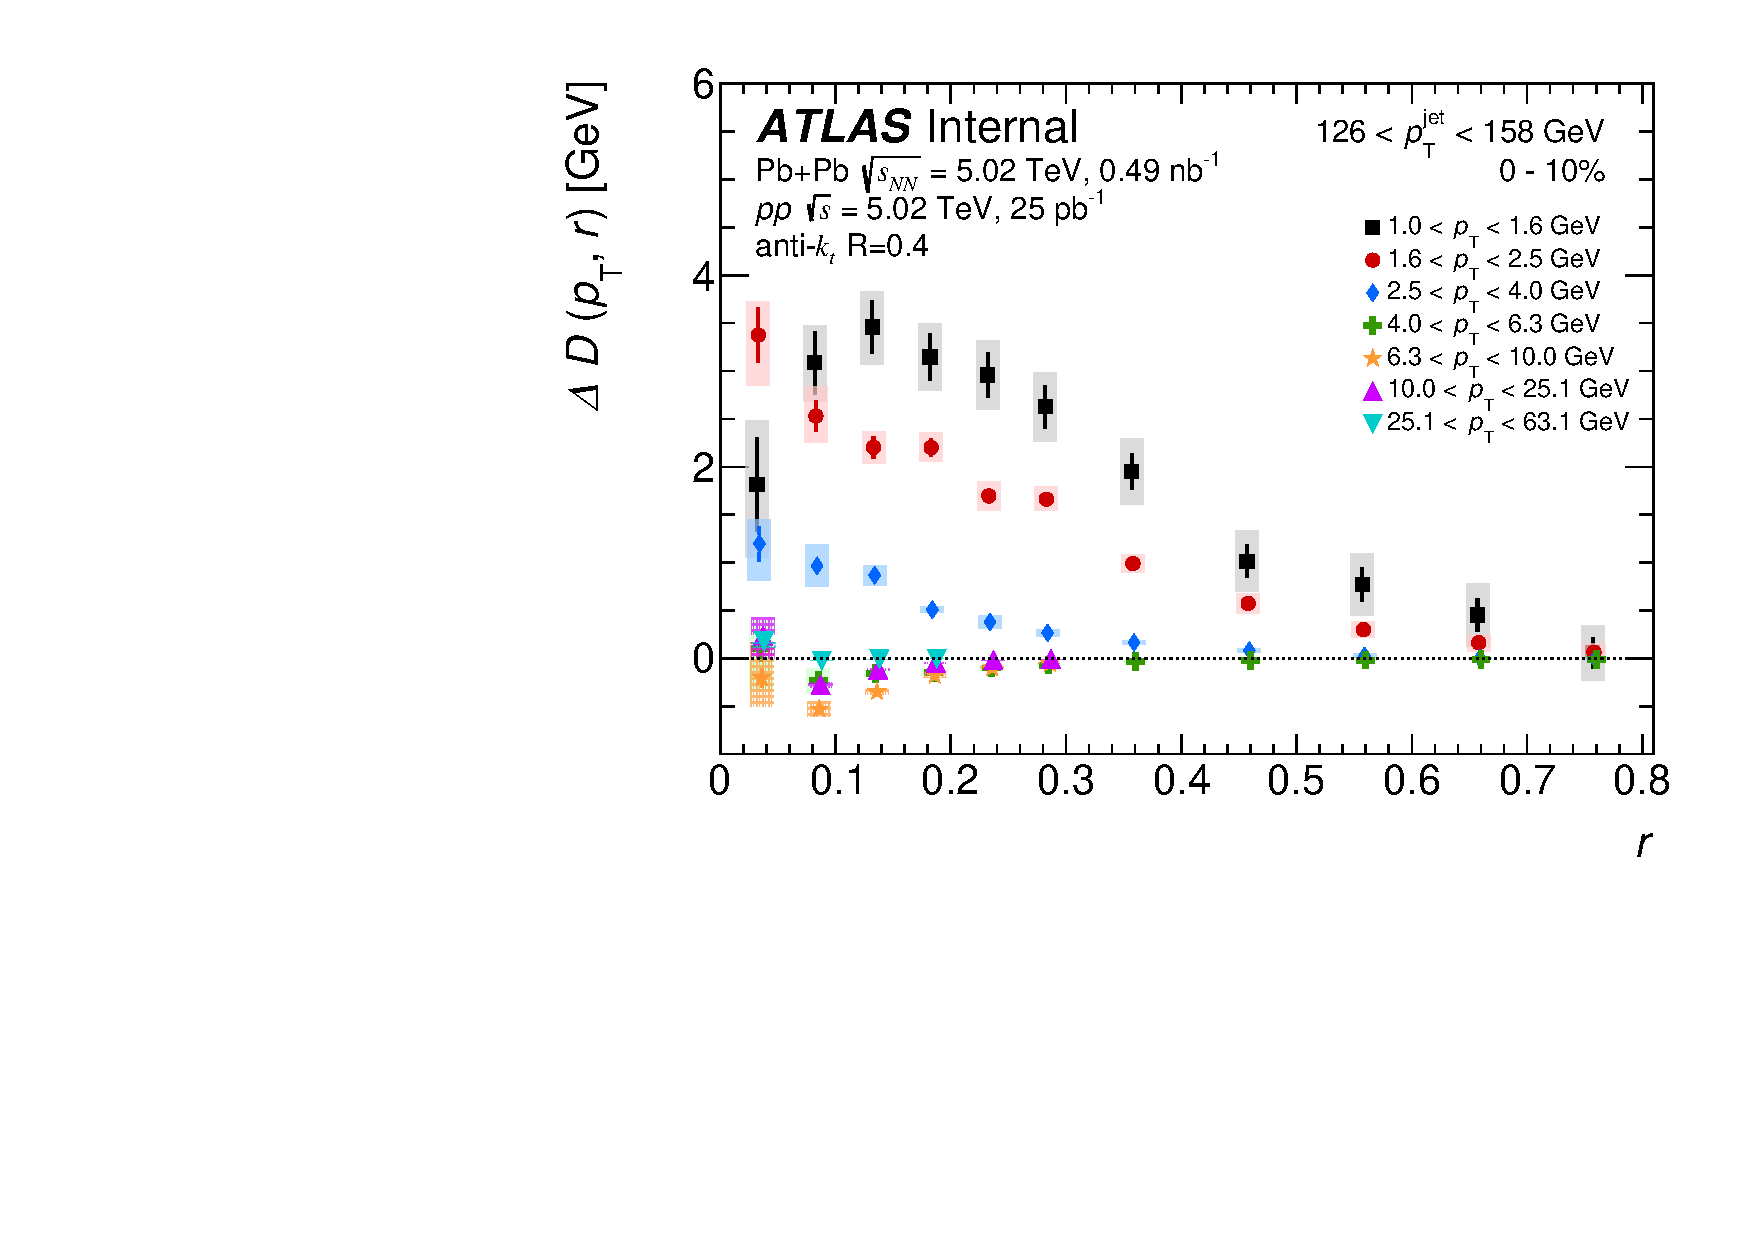
\includegraphics[width=0.45\textwidth]{results/DeltaDpT_final_ratio_dR_CONF_data_jet7_cent0} &
	 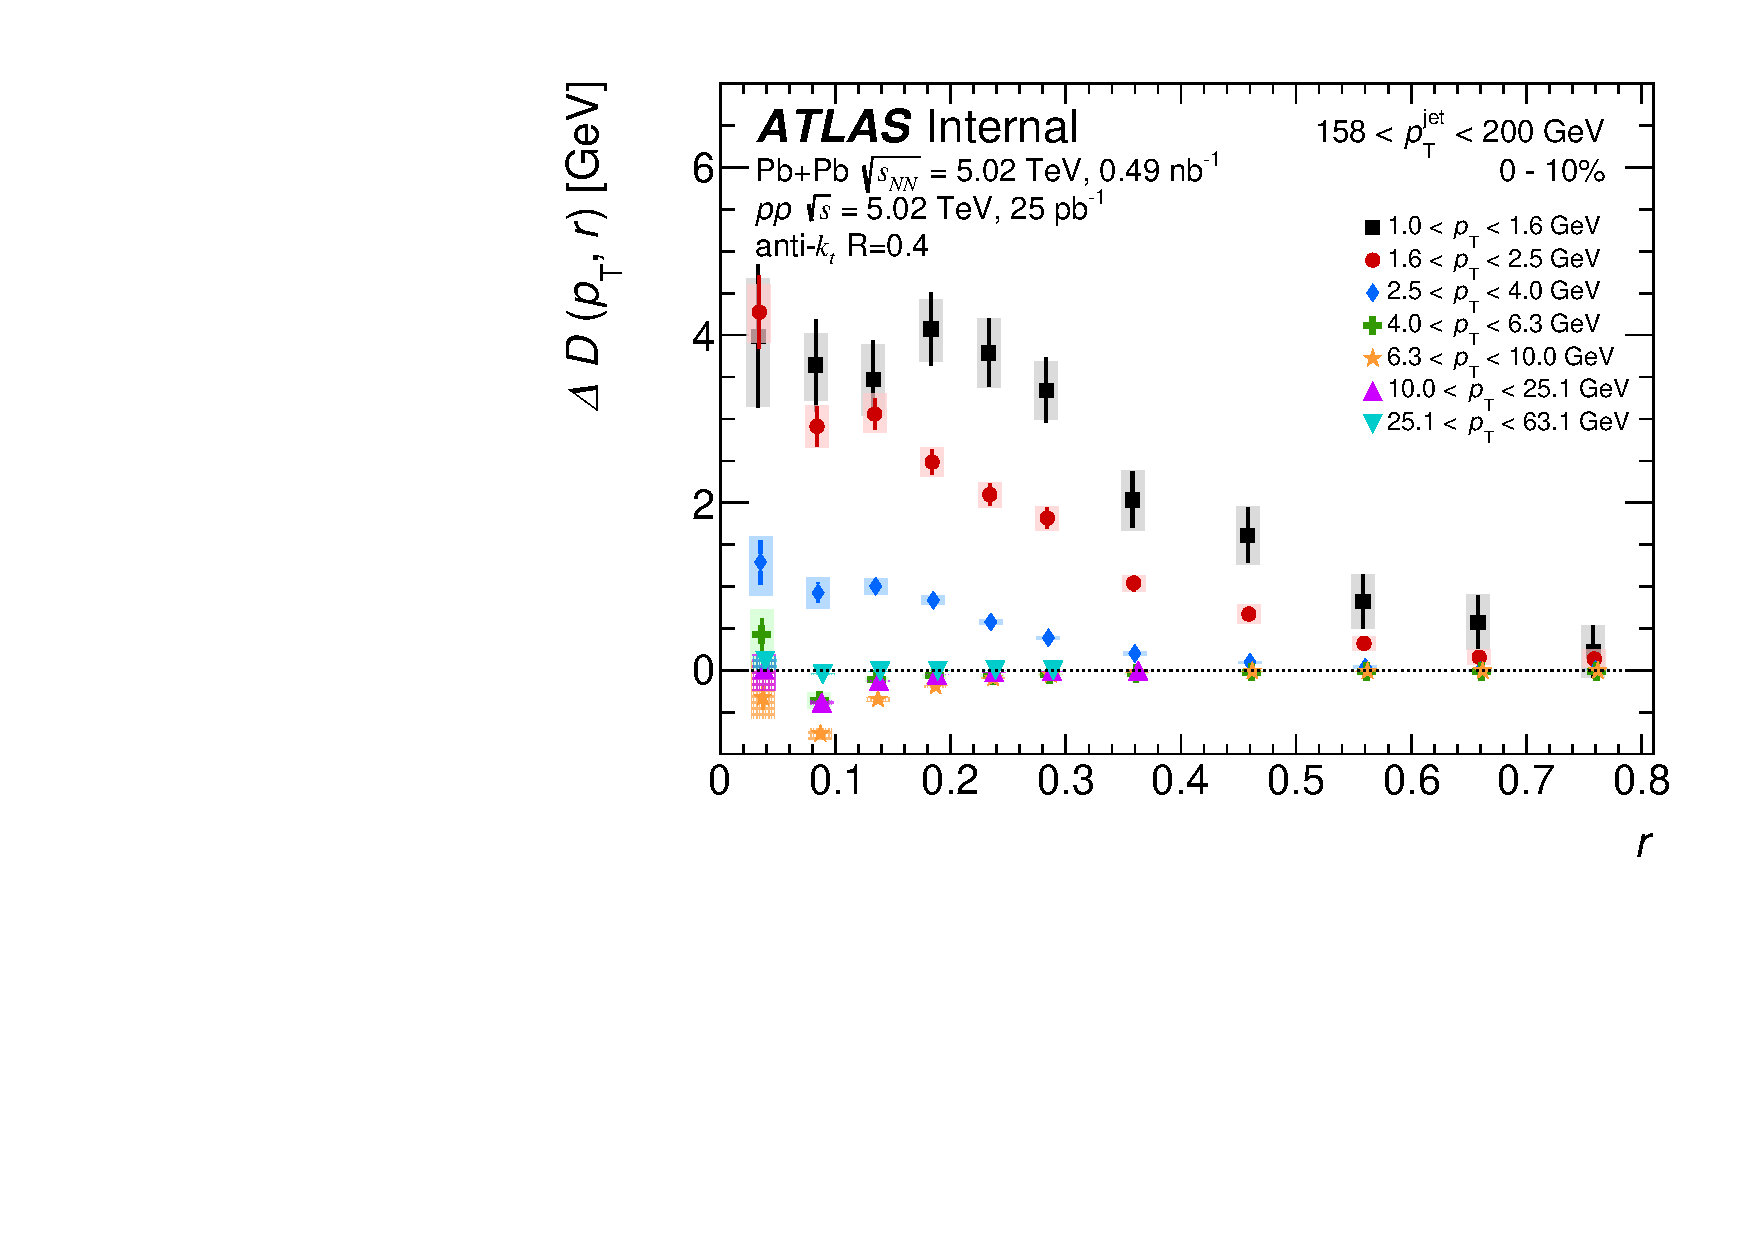
\includegraphics[width=0.45\textwidth]{results/DeltaDpT_final_ratio_dR_CONF_data_jet8_cent0} \\
	 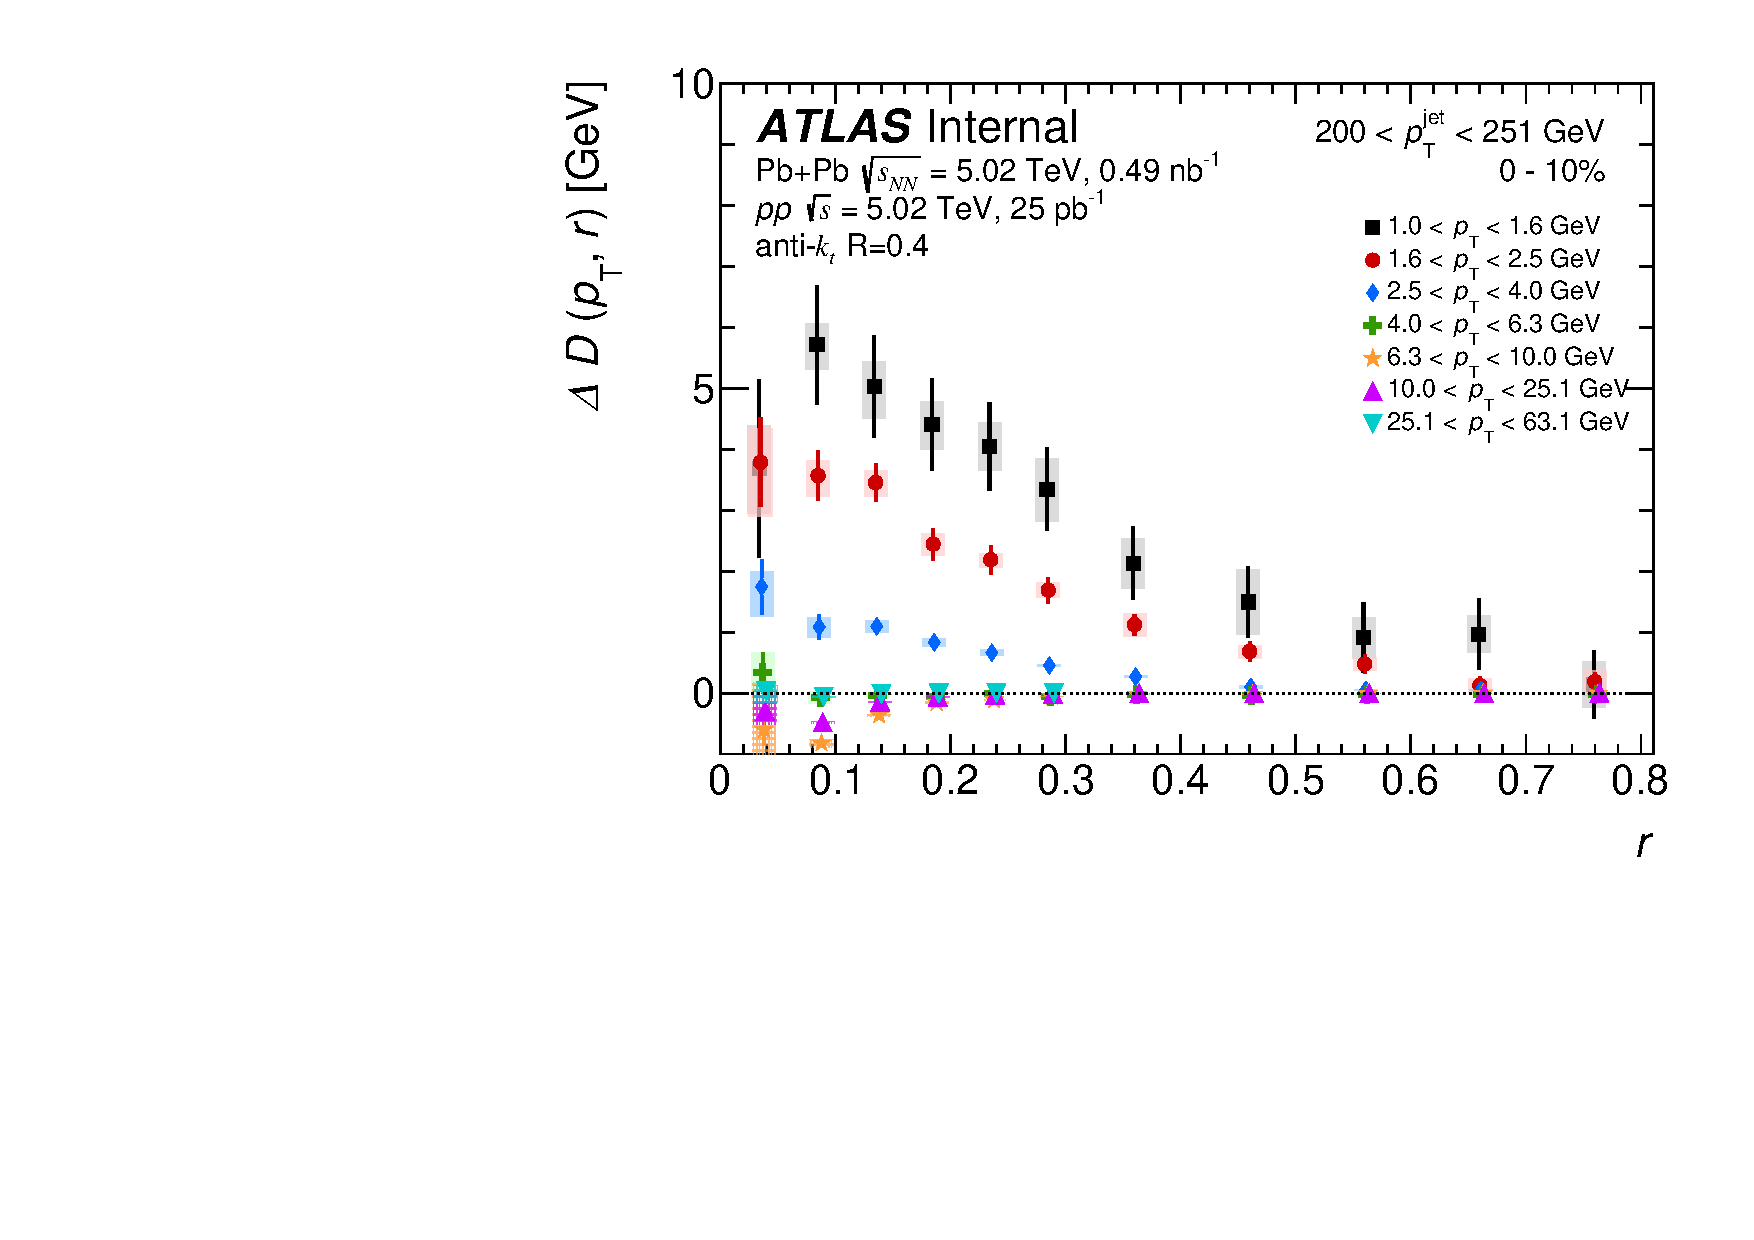
\includegraphics[width=0.45\textwidth]{results/DeltaDpT_final_ratio_dR_CONF_data_jet9_cent0} &
	 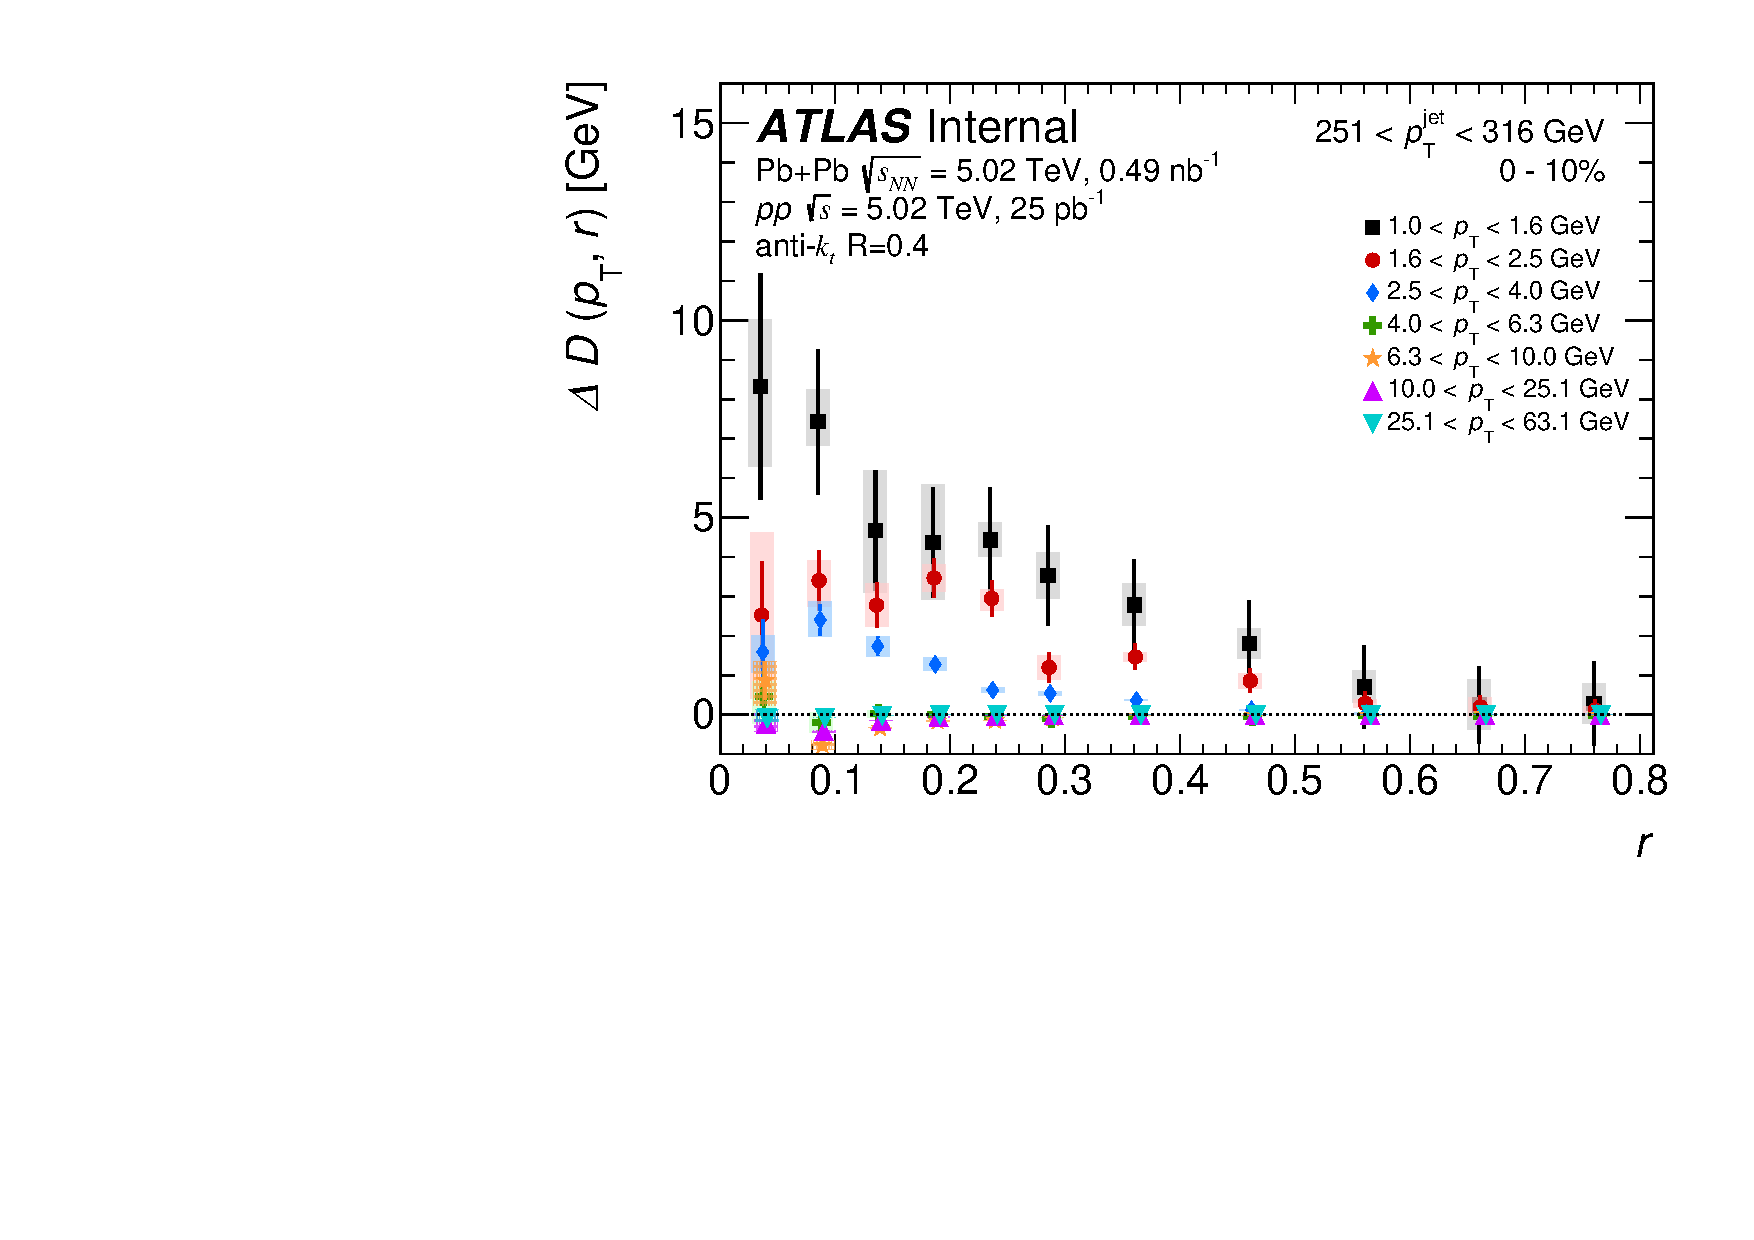
\includegraphics[width=0.45\textwidth]{results/DeltaDpT_final_ratio_dR_CONF_data_jet10_cent0} \\
\end{tabular} }
   \caption{$\Delta \RDptr$ as a function of \rvar\ in central collisions for all \pt\ ranges in four \ptjet\ selections: 126--158~\GeV, 158--200~\GeV, 200--251~\GeV, and 251--316~\GeV. }
      \label{fig:deltadptr}
\end{figure}


\begin{figure}
\centering{
\begin{tabular}{cc}
	 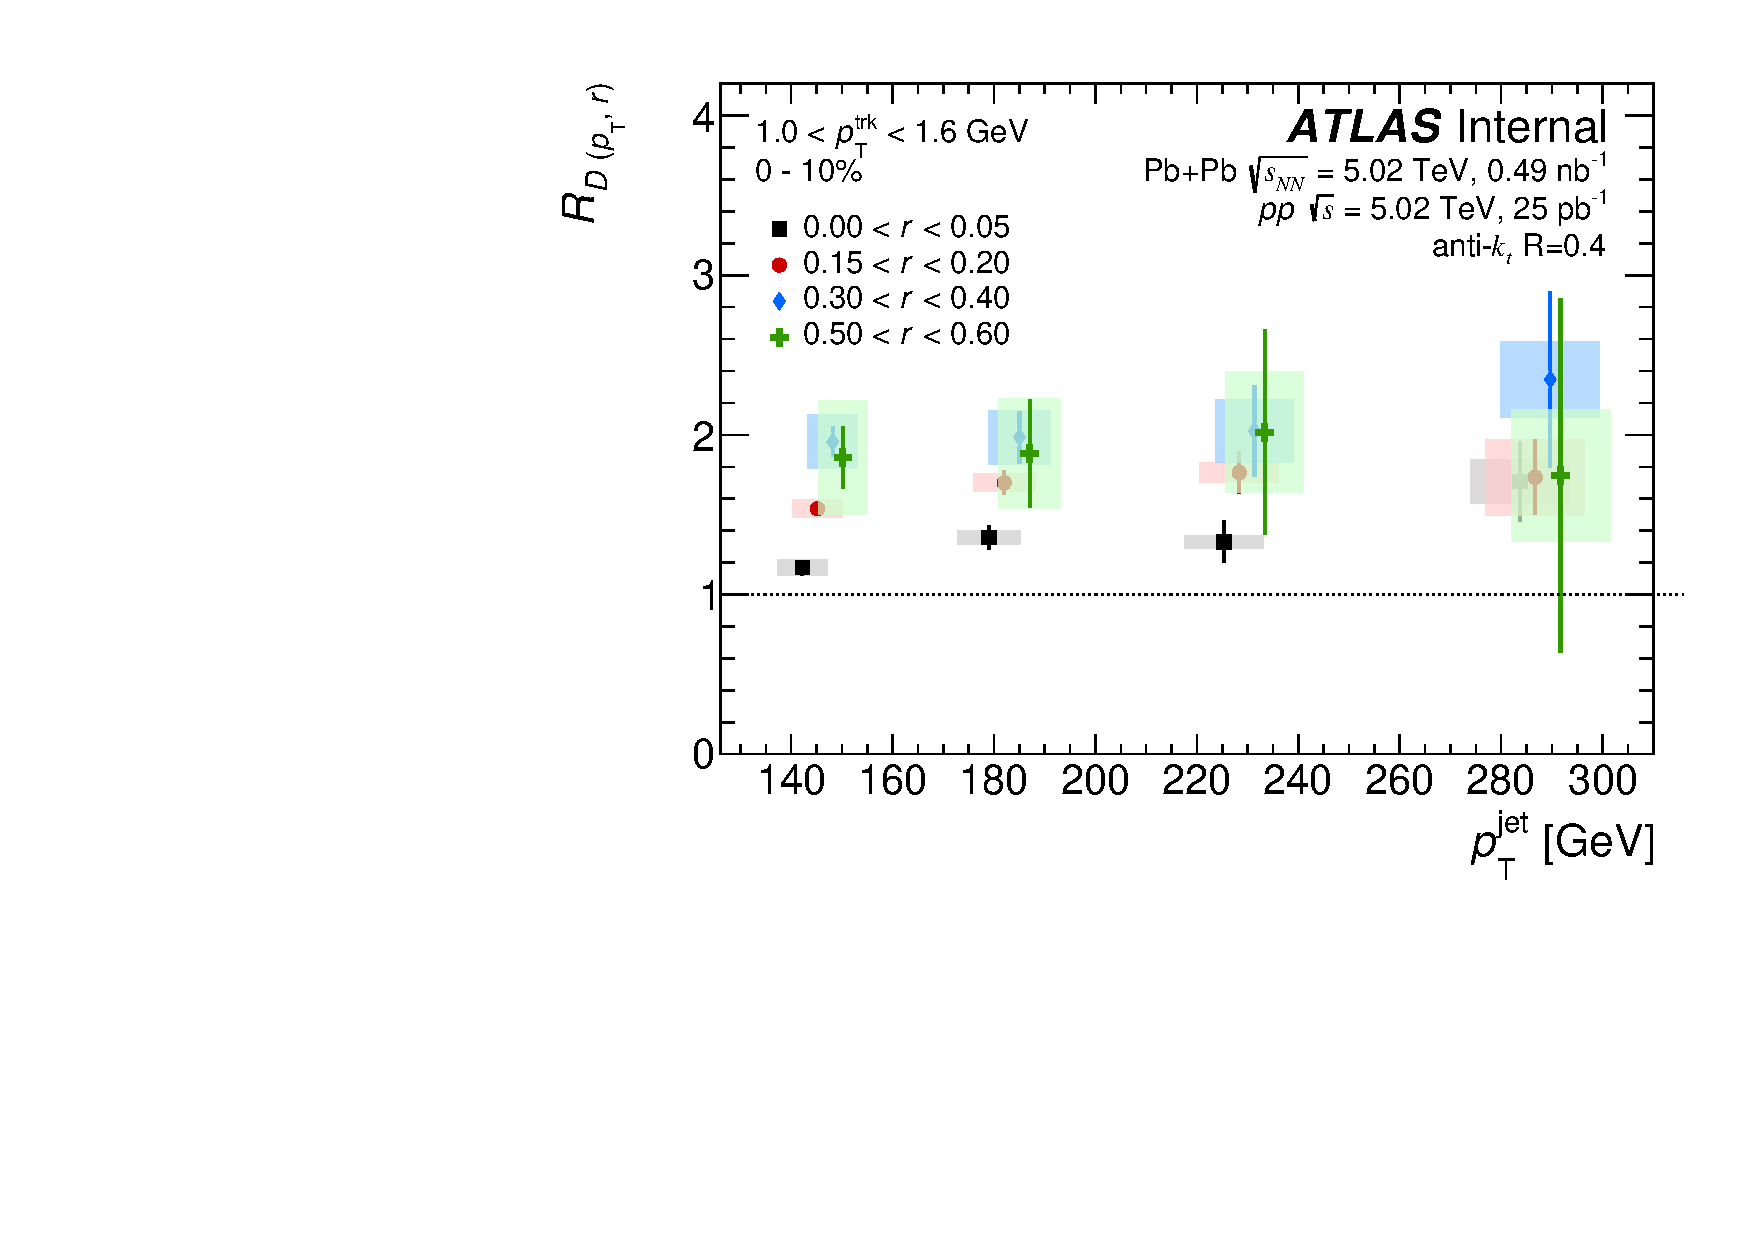
\includegraphics[width=0.45\textwidth]{results/zRDpT_final_ratio_dR_CONF_data_jetpT_trk2_cent0} &
	 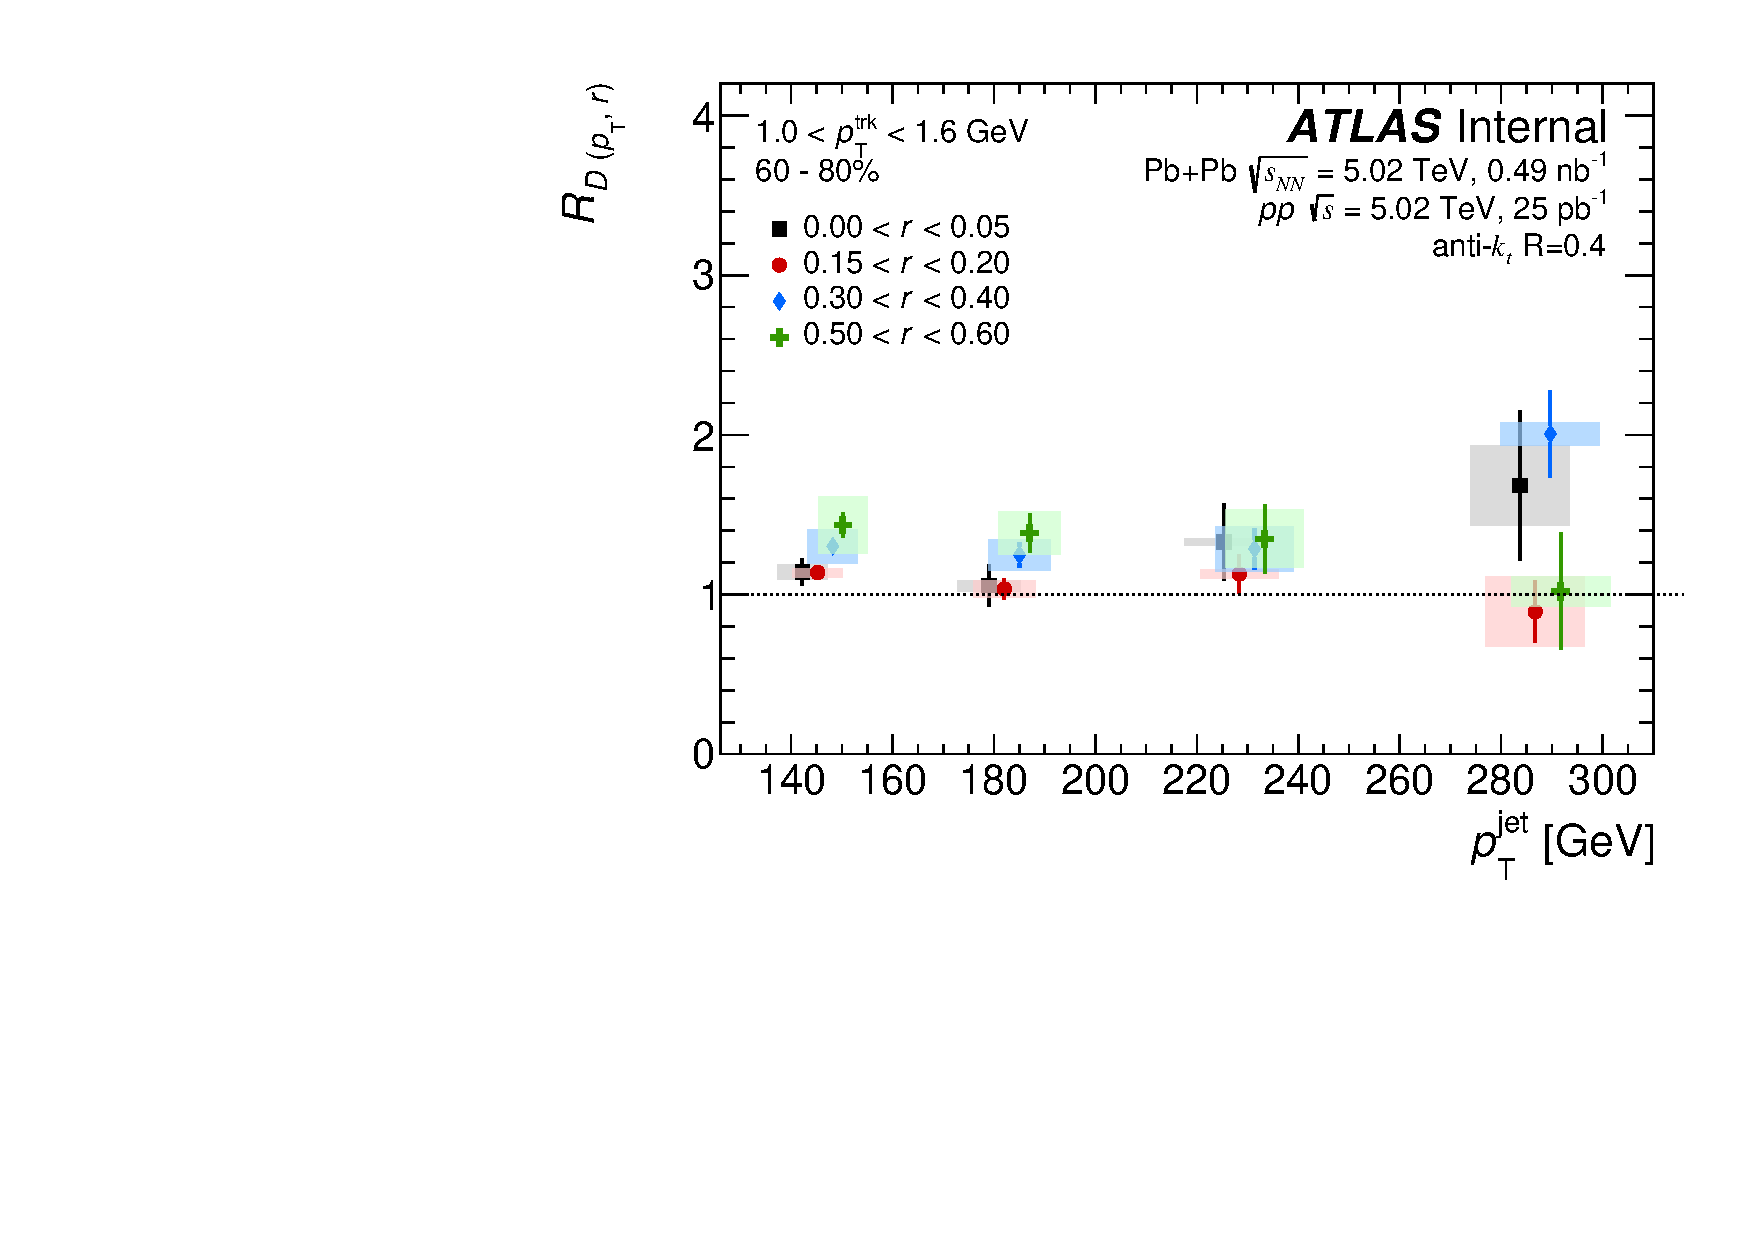
\includegraphics[width=0.45\textwidth]{results/zRDpT_final_ratio_dR_CONF_data_jetpT_trk2_cent5} \\
	 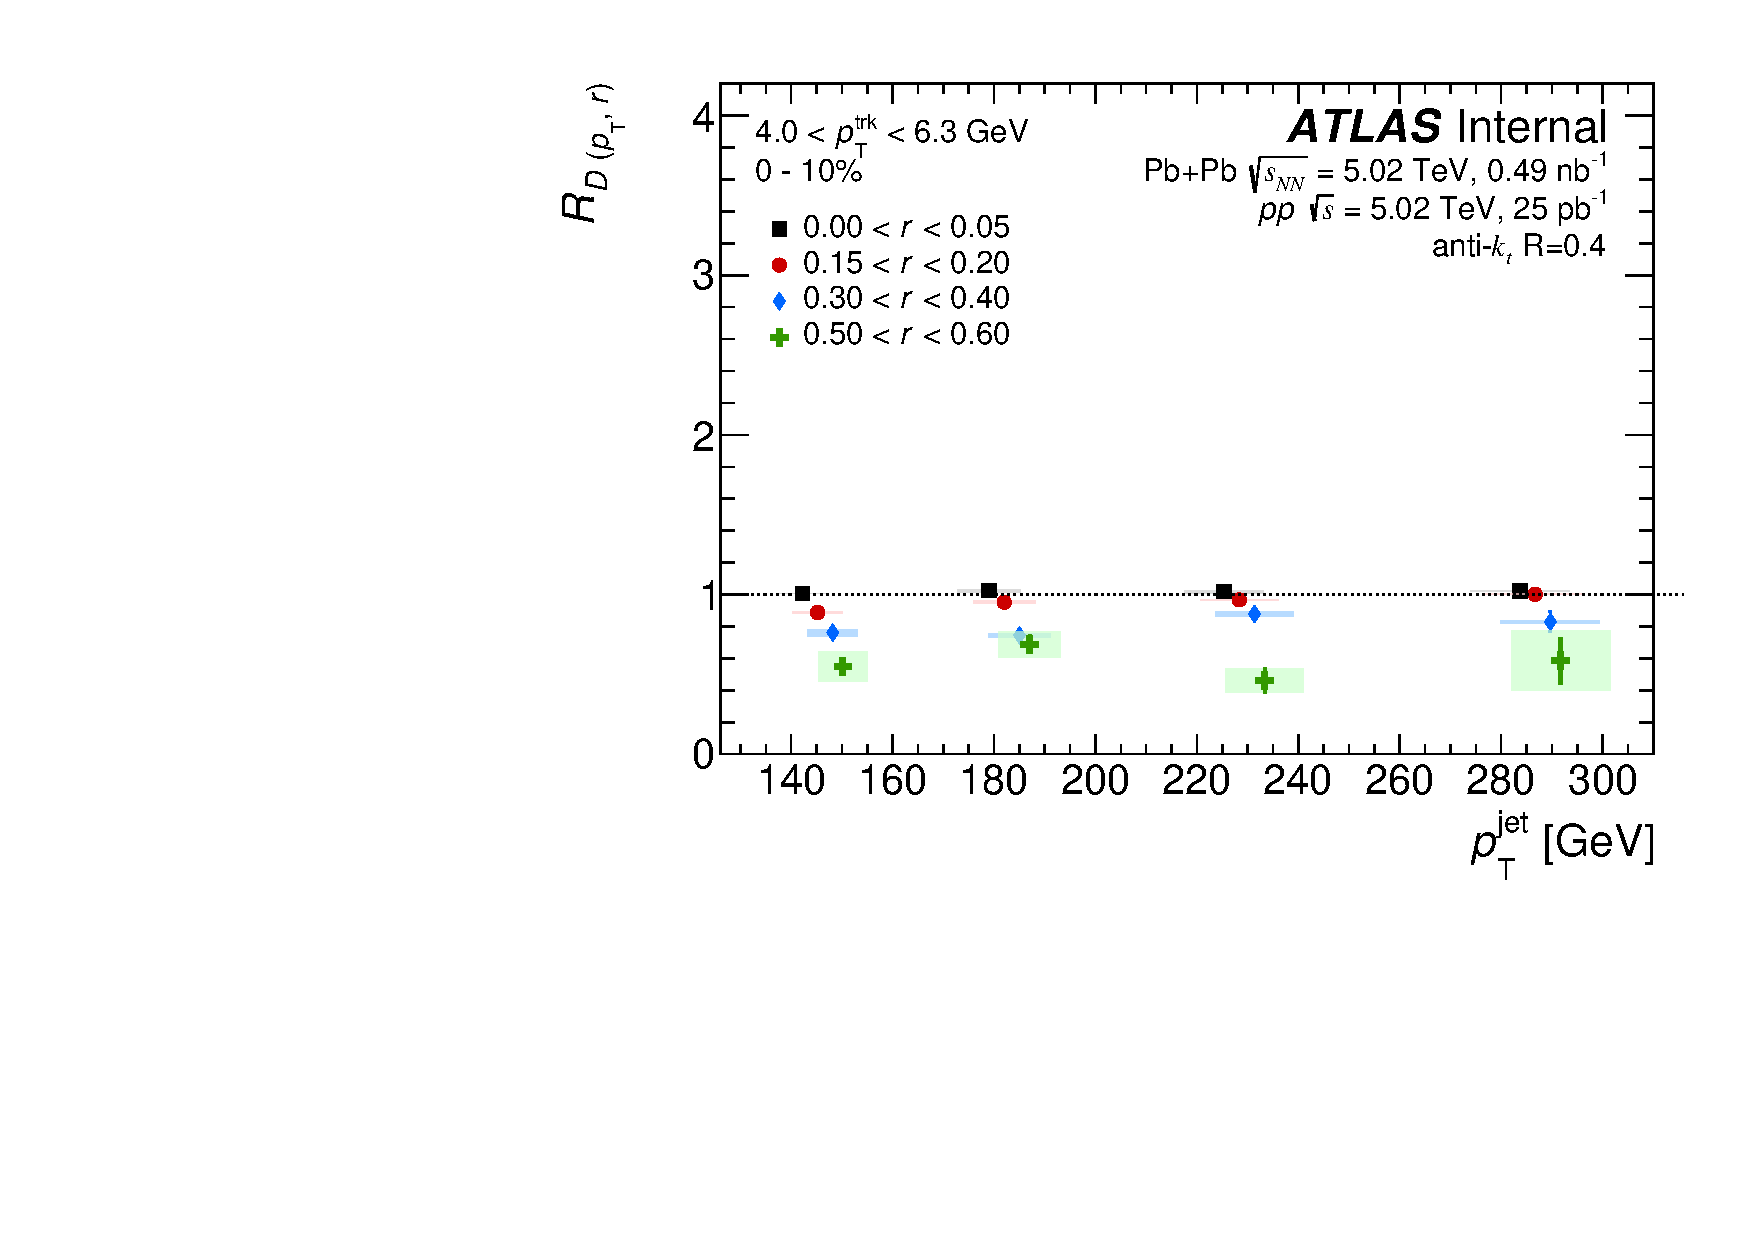
\includegraphics[width=0.45\textwidth]{results/zRDpT_final_ratio_dR_CONF_data_jetpT_trk5_cent0} &
	 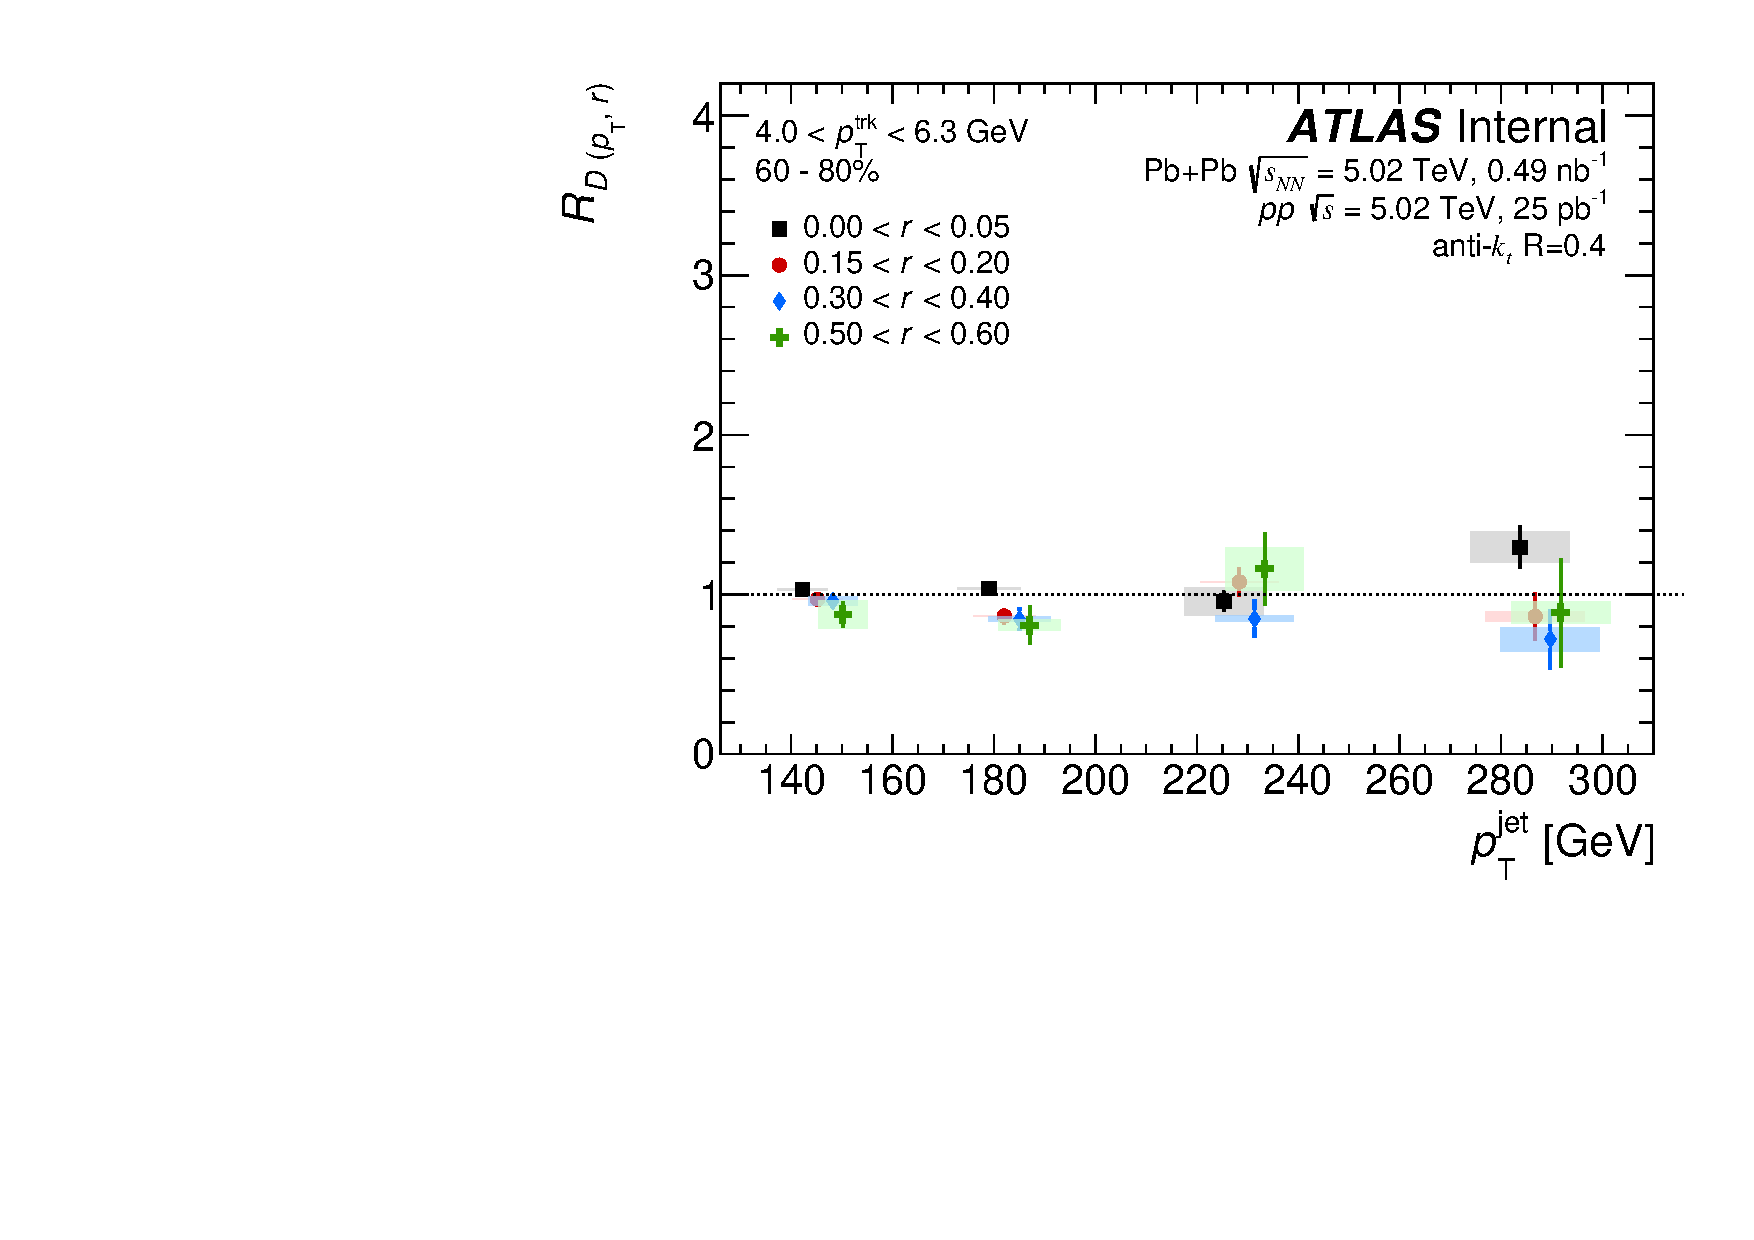
\includegraphics[width=0.45\textwidth]{results/zRDpT_final_ratio_dR_CONF_data_jetpT_trk5_cent5} \\
\end{tabular} }
   \caption{\RDptr as a function of \ptjet\ for charged particles with $1.0 < \pt < 1.6$ GeV (top) and $4.0 < \pt < 6.3$ GeV (bottom) at different distances from the jet axis and in 0--10\% central (left) and 60--80\% peripheral (right) \pbpb\ collisions.}
      \label{fig:rdptr_jetpt}
\end{figure}



\begin{figure}
\centering{
\begin{tabular}{cc}
	 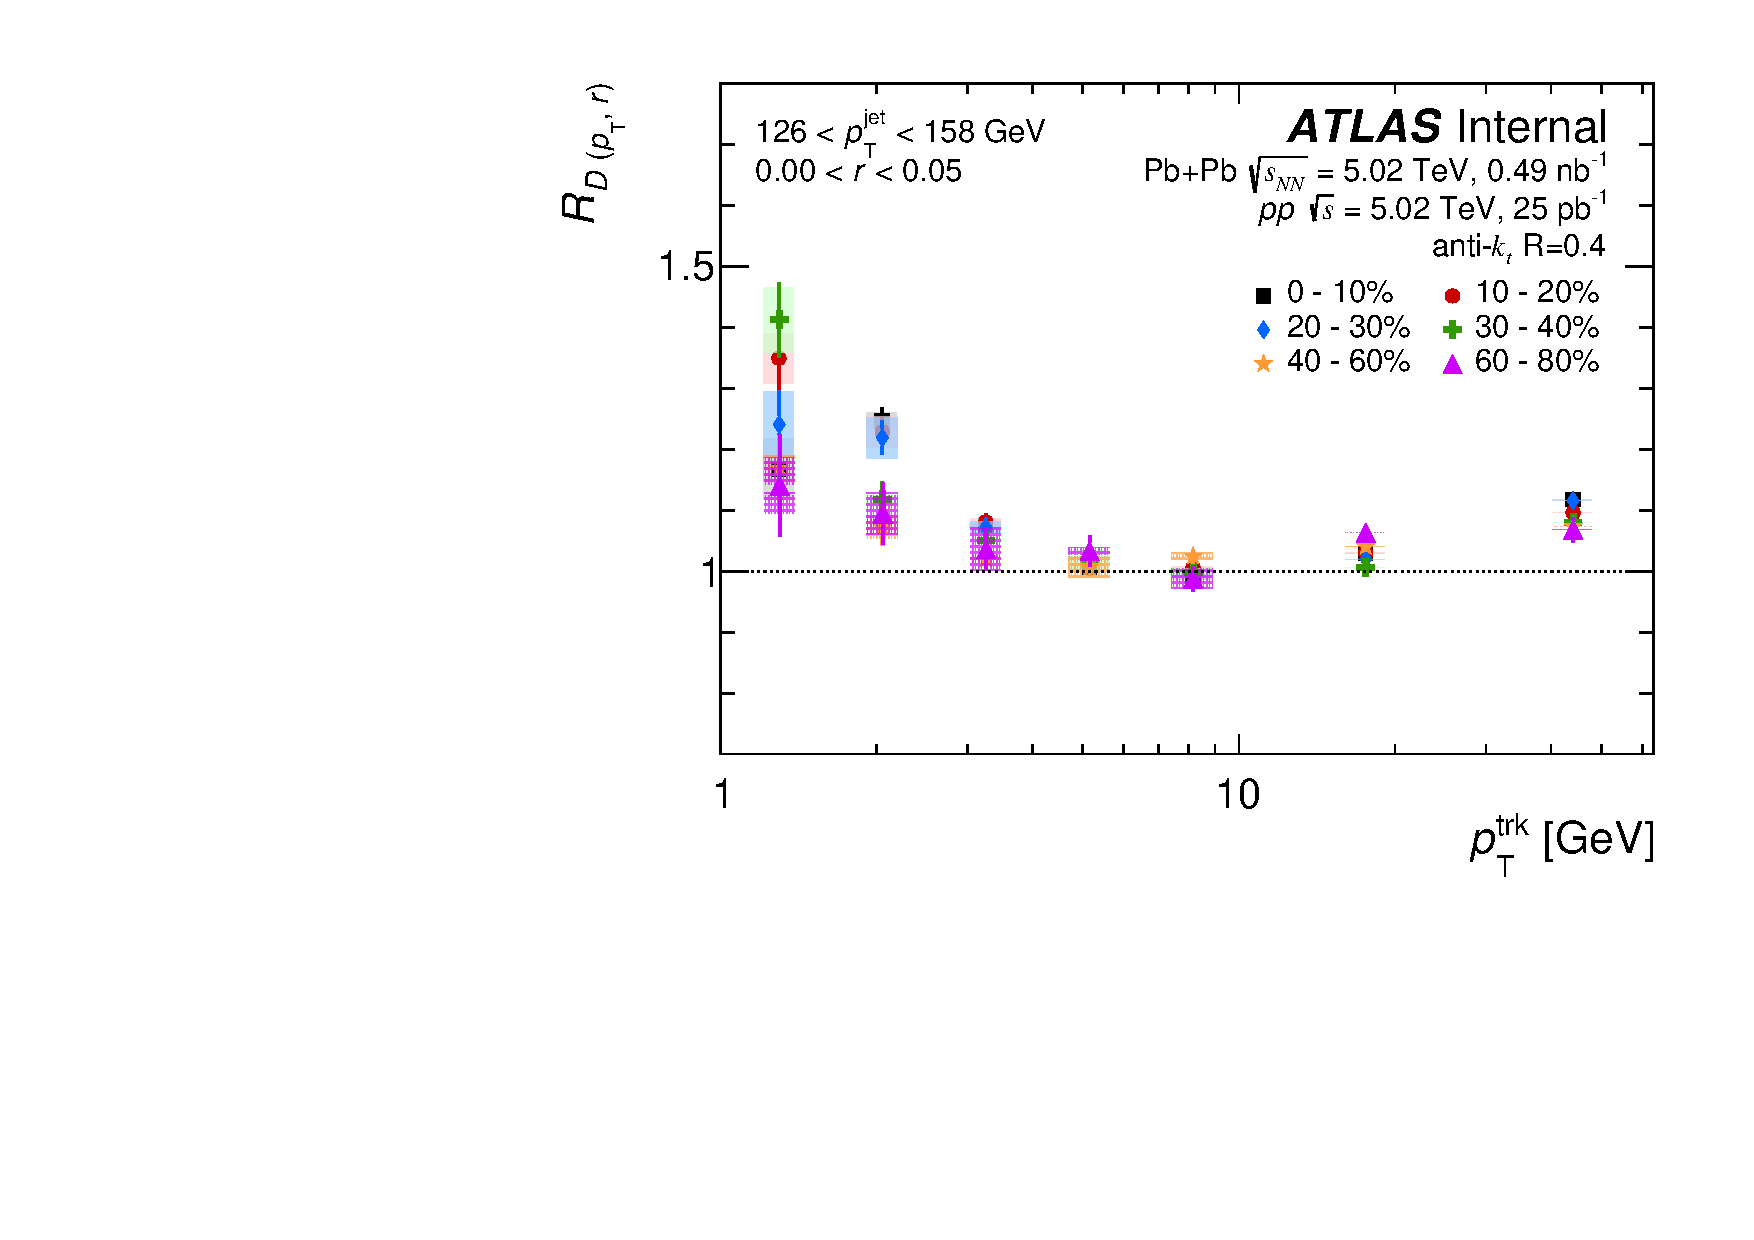
\includegraphics[width=0.5\textwidth]{results/xRDpT_final_ratio_dR_CONF_data_trkpT_jet7_dR0} &
	 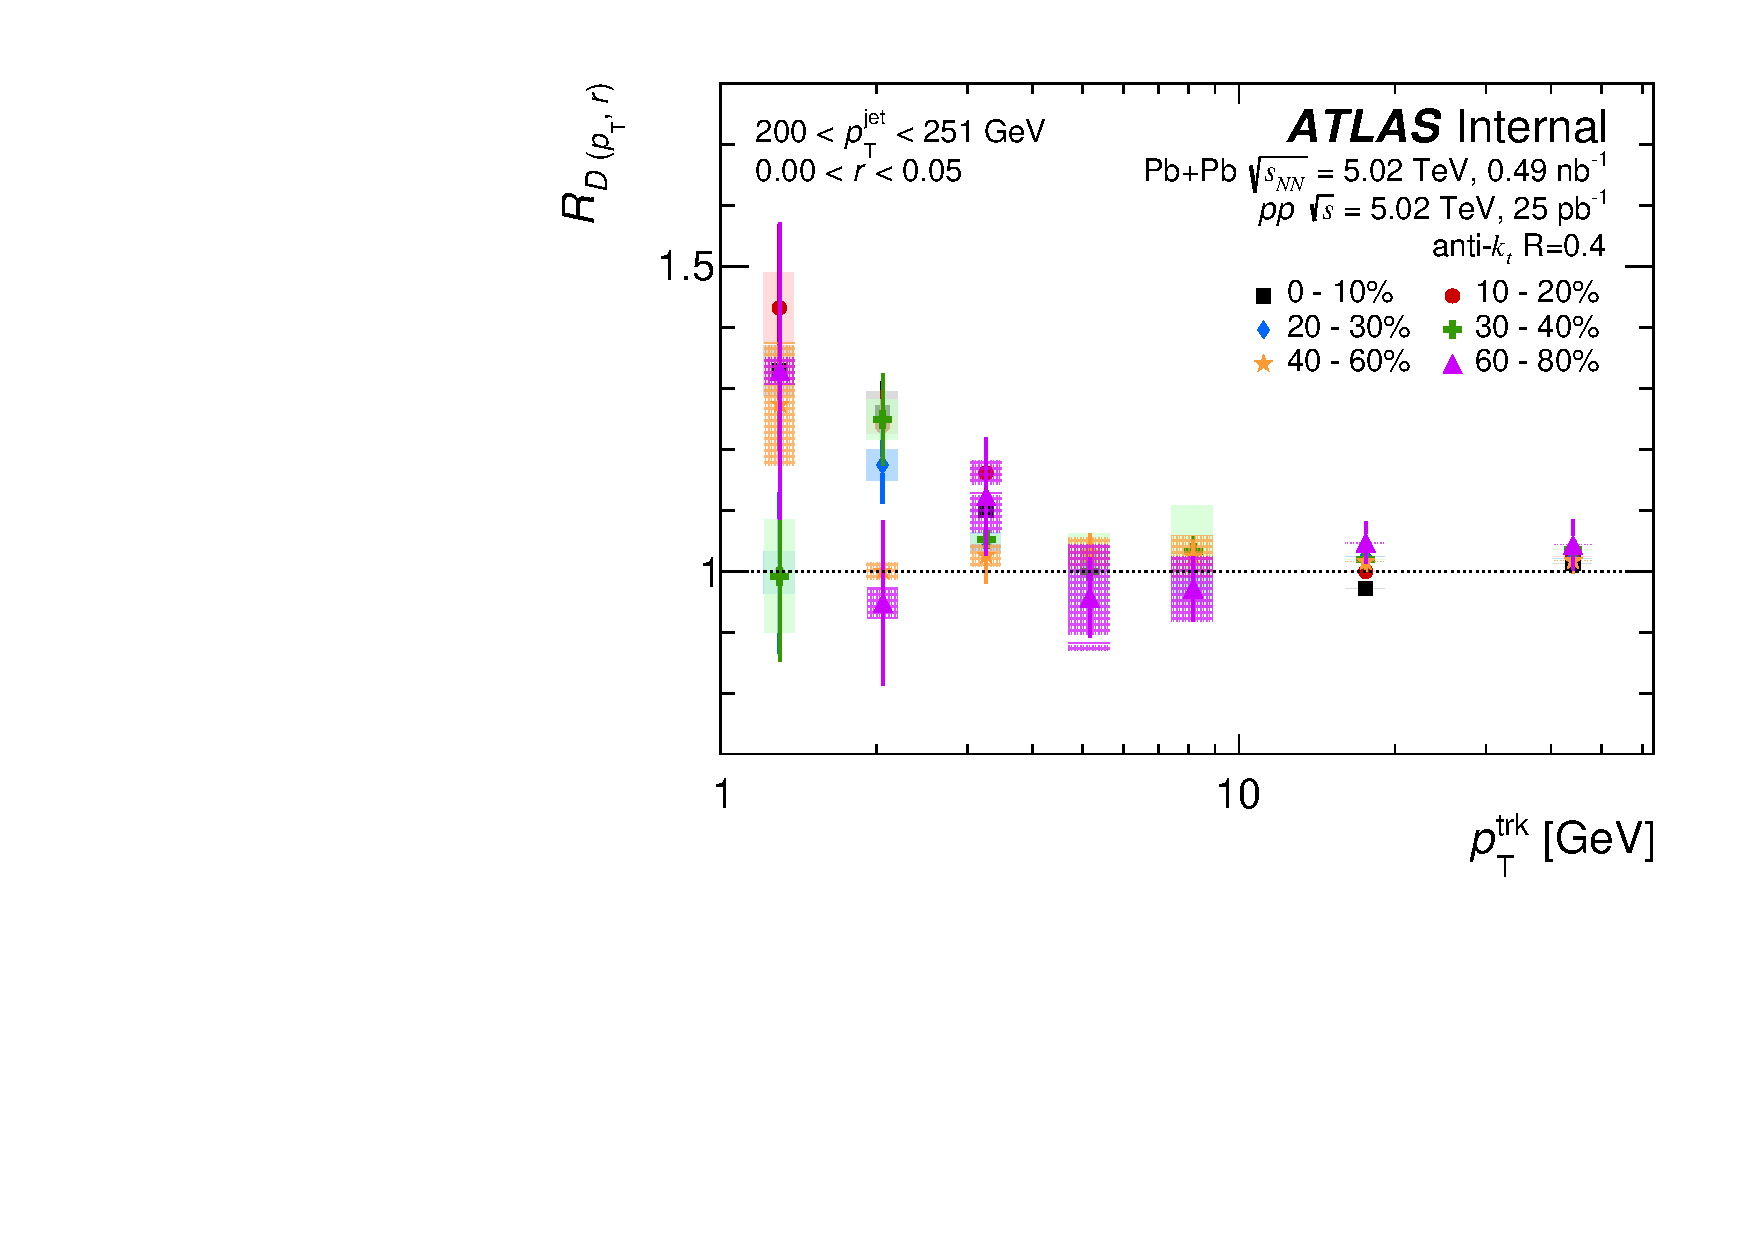
\includegraphics[width=0.5\textwidth]{results/xRDpT_final_ratio_dR_CONF_data_trkpT_jet9_dR0} \\
	 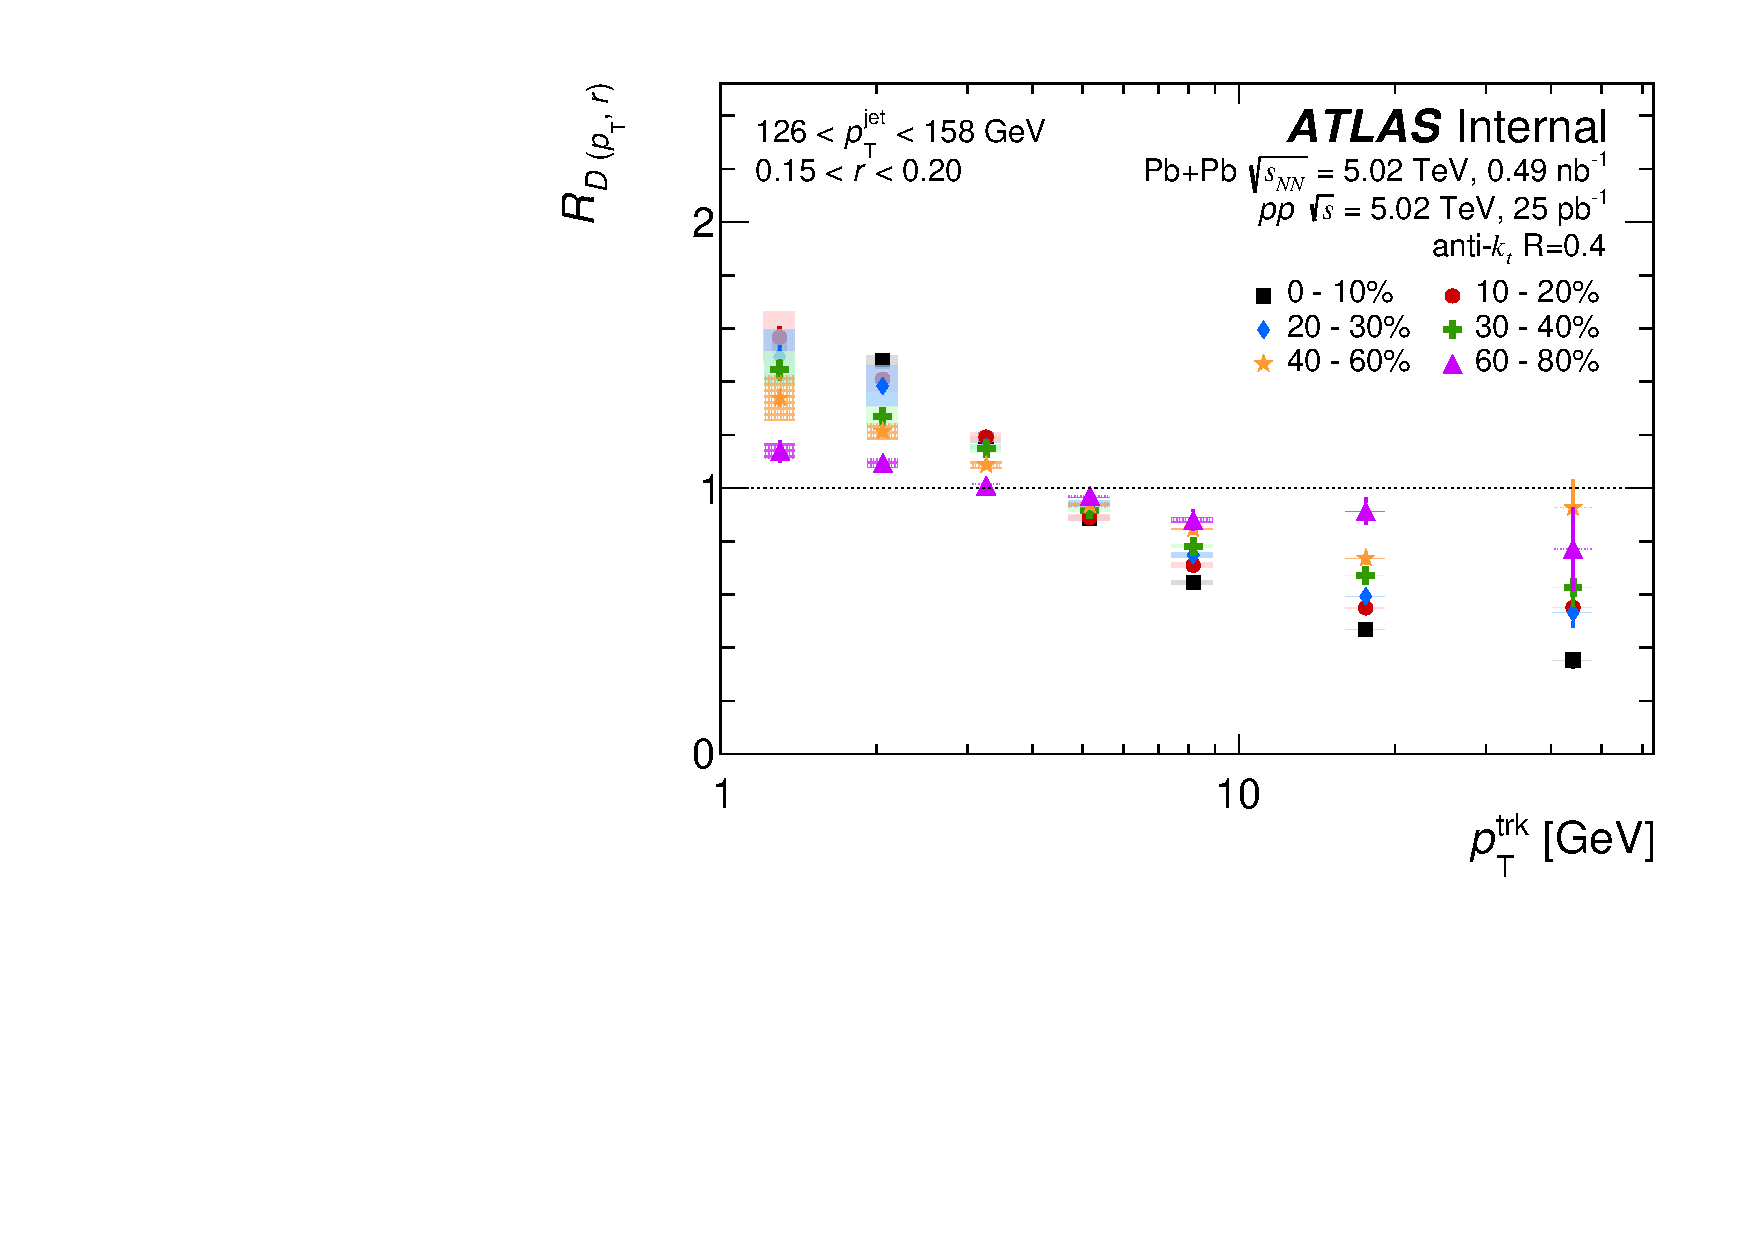
\includegraphics[width=0.5\textwidth]{results/xRDpT_final_ratio_dR_CONF_data_trkpT_jet7_dR3} &
	 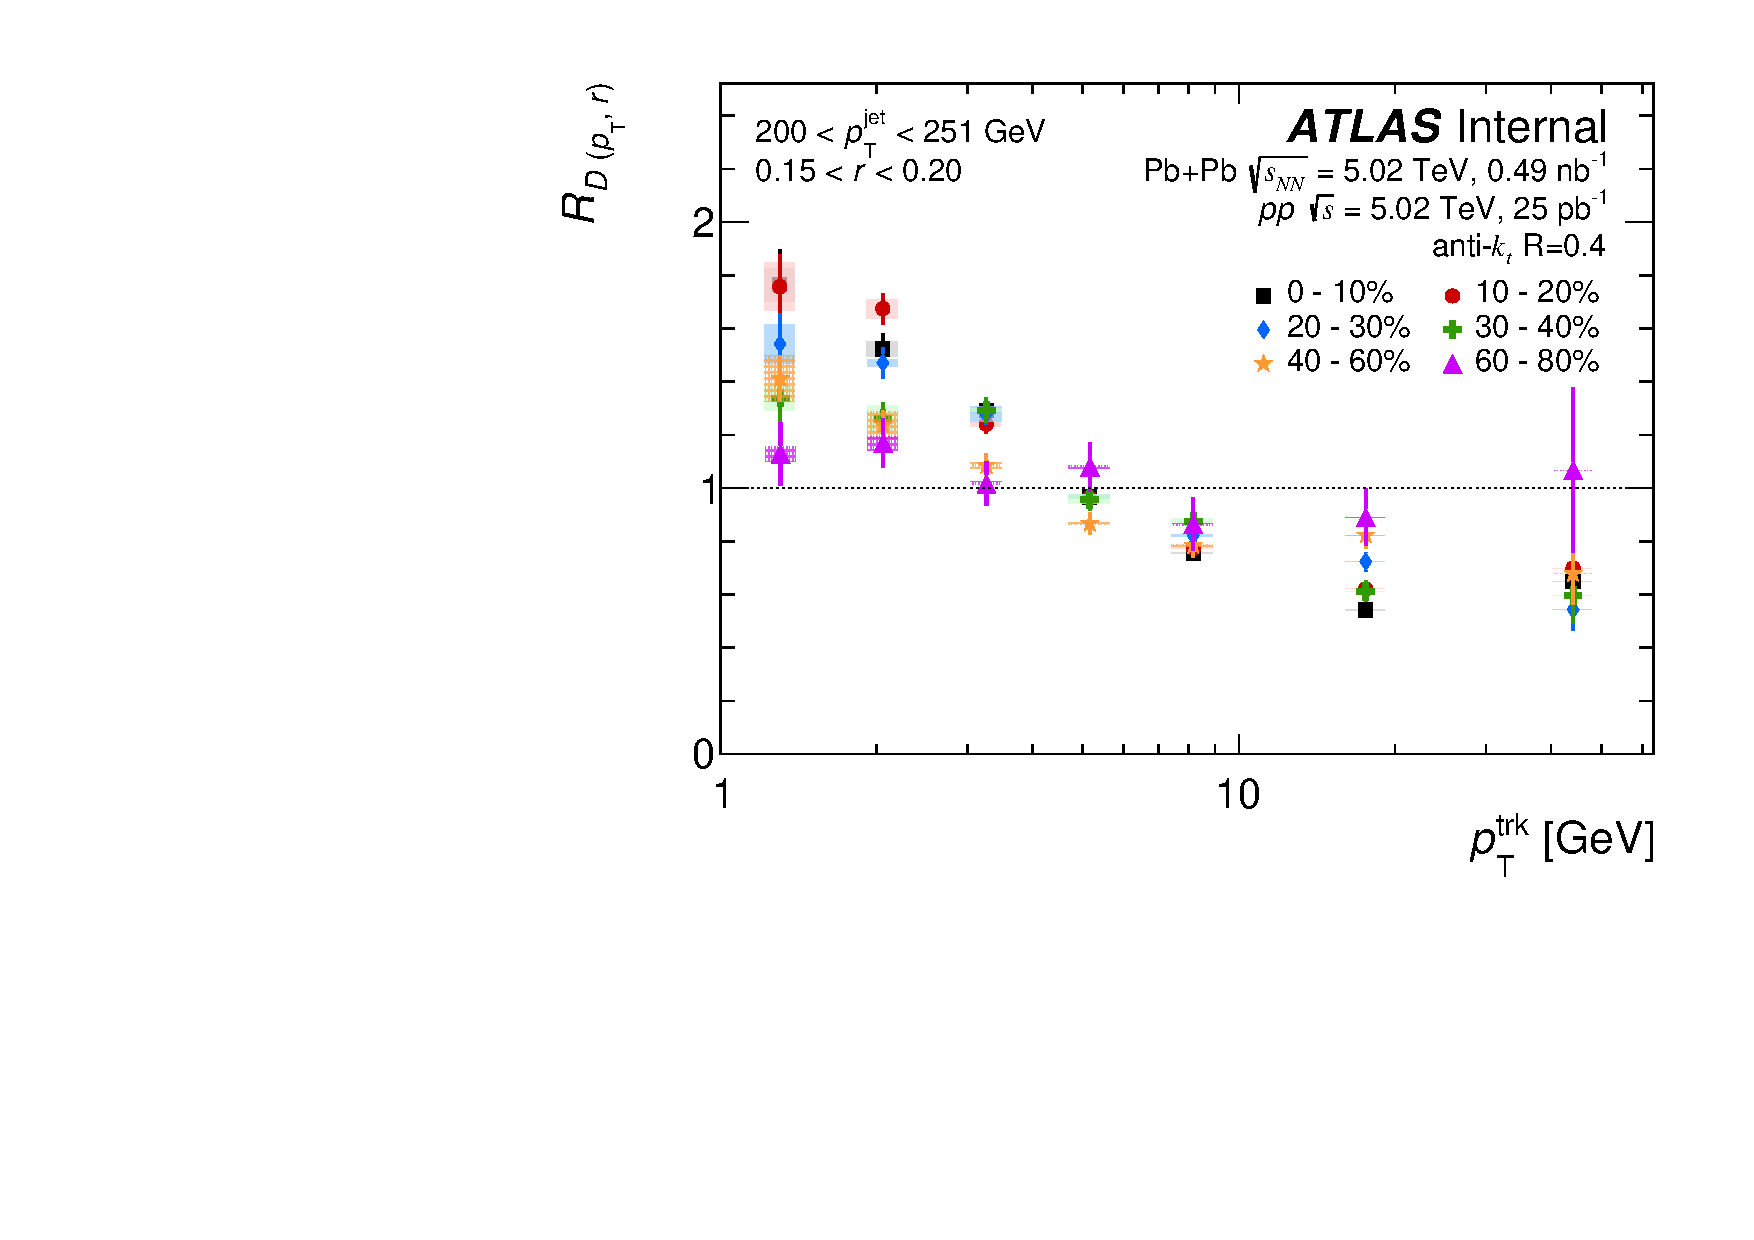
\includegraphics[width=0.5\textwidth]{results/xRDpT_final_ratio_dR_CONF_data_trkpT_jet9_dR3} \\
	 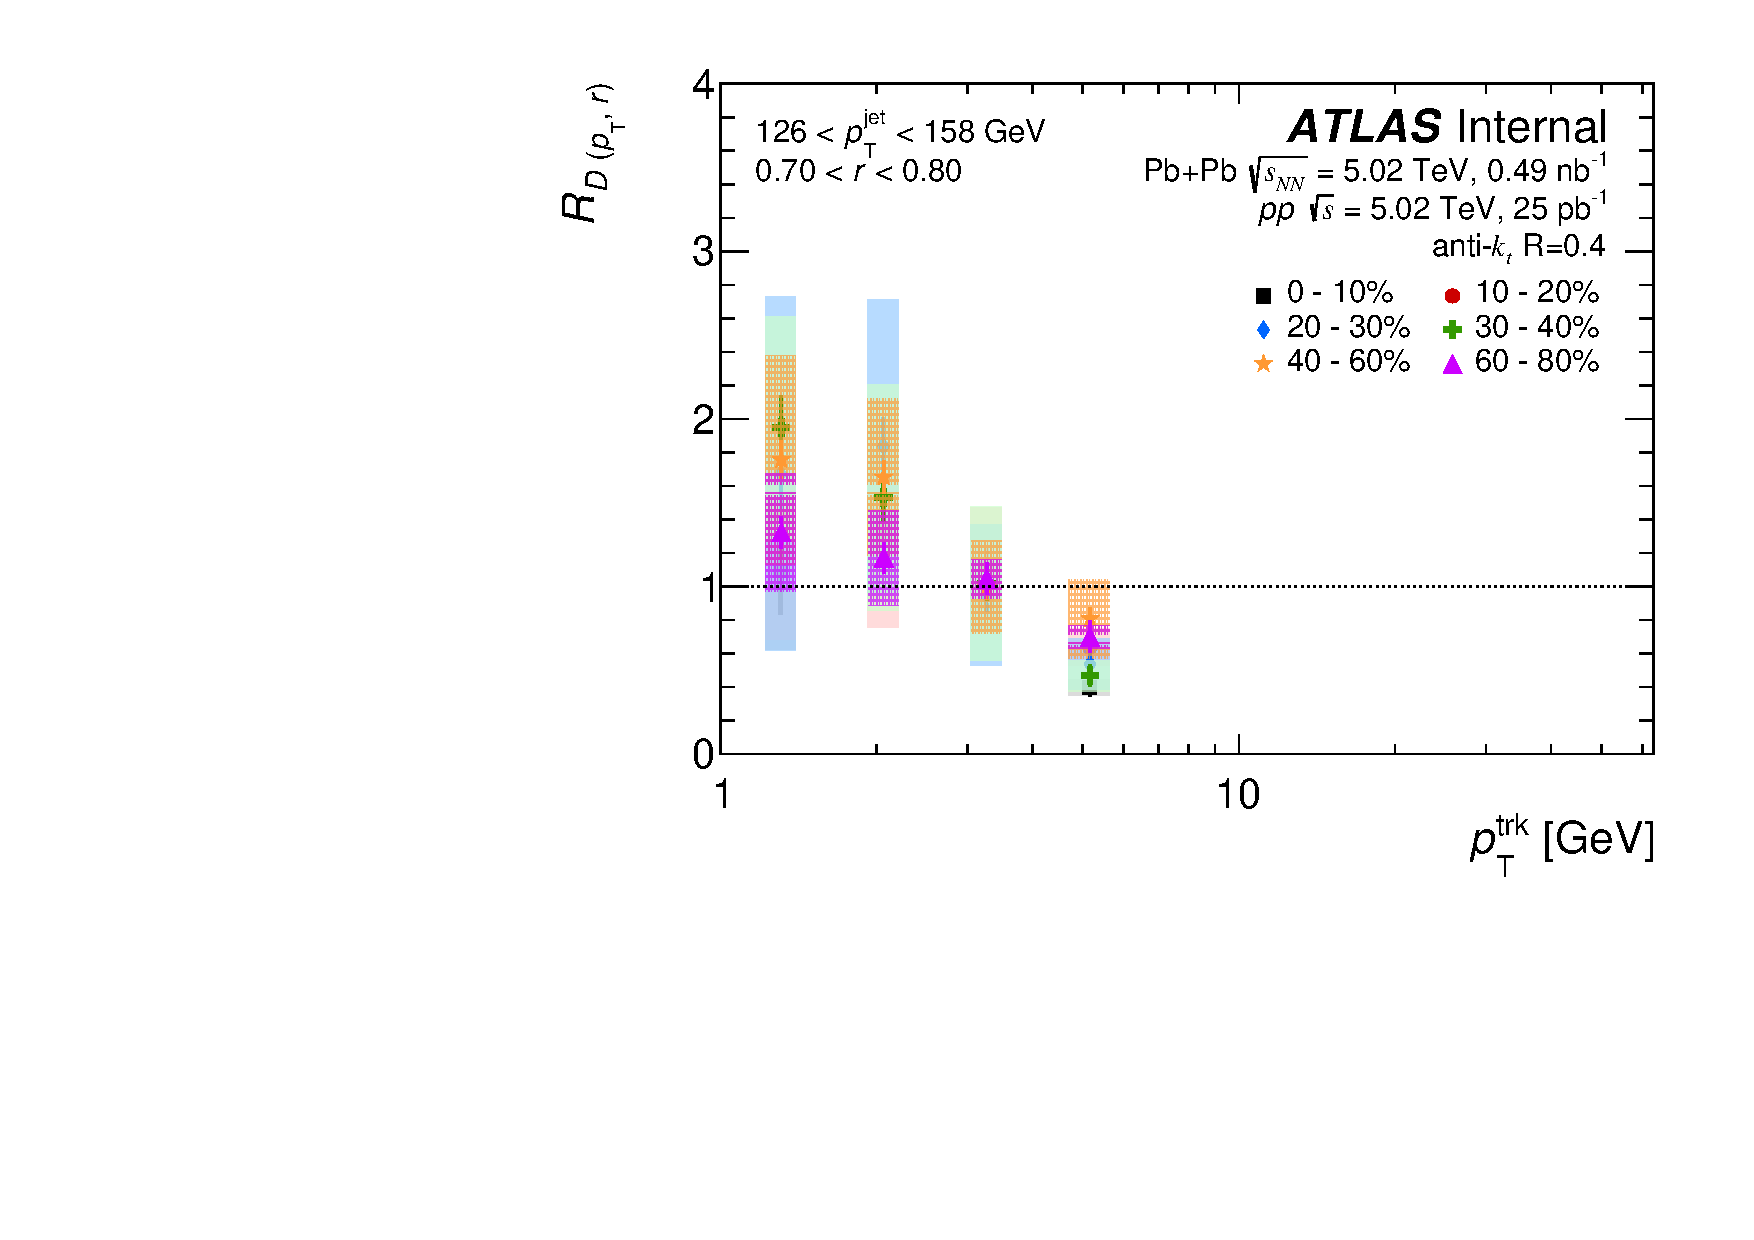
\includegraphics[width=0.5\textwidth]{results/xRDpT_final_ratio_dR_CONF_data_trkpT_jet7_dR10} &
	 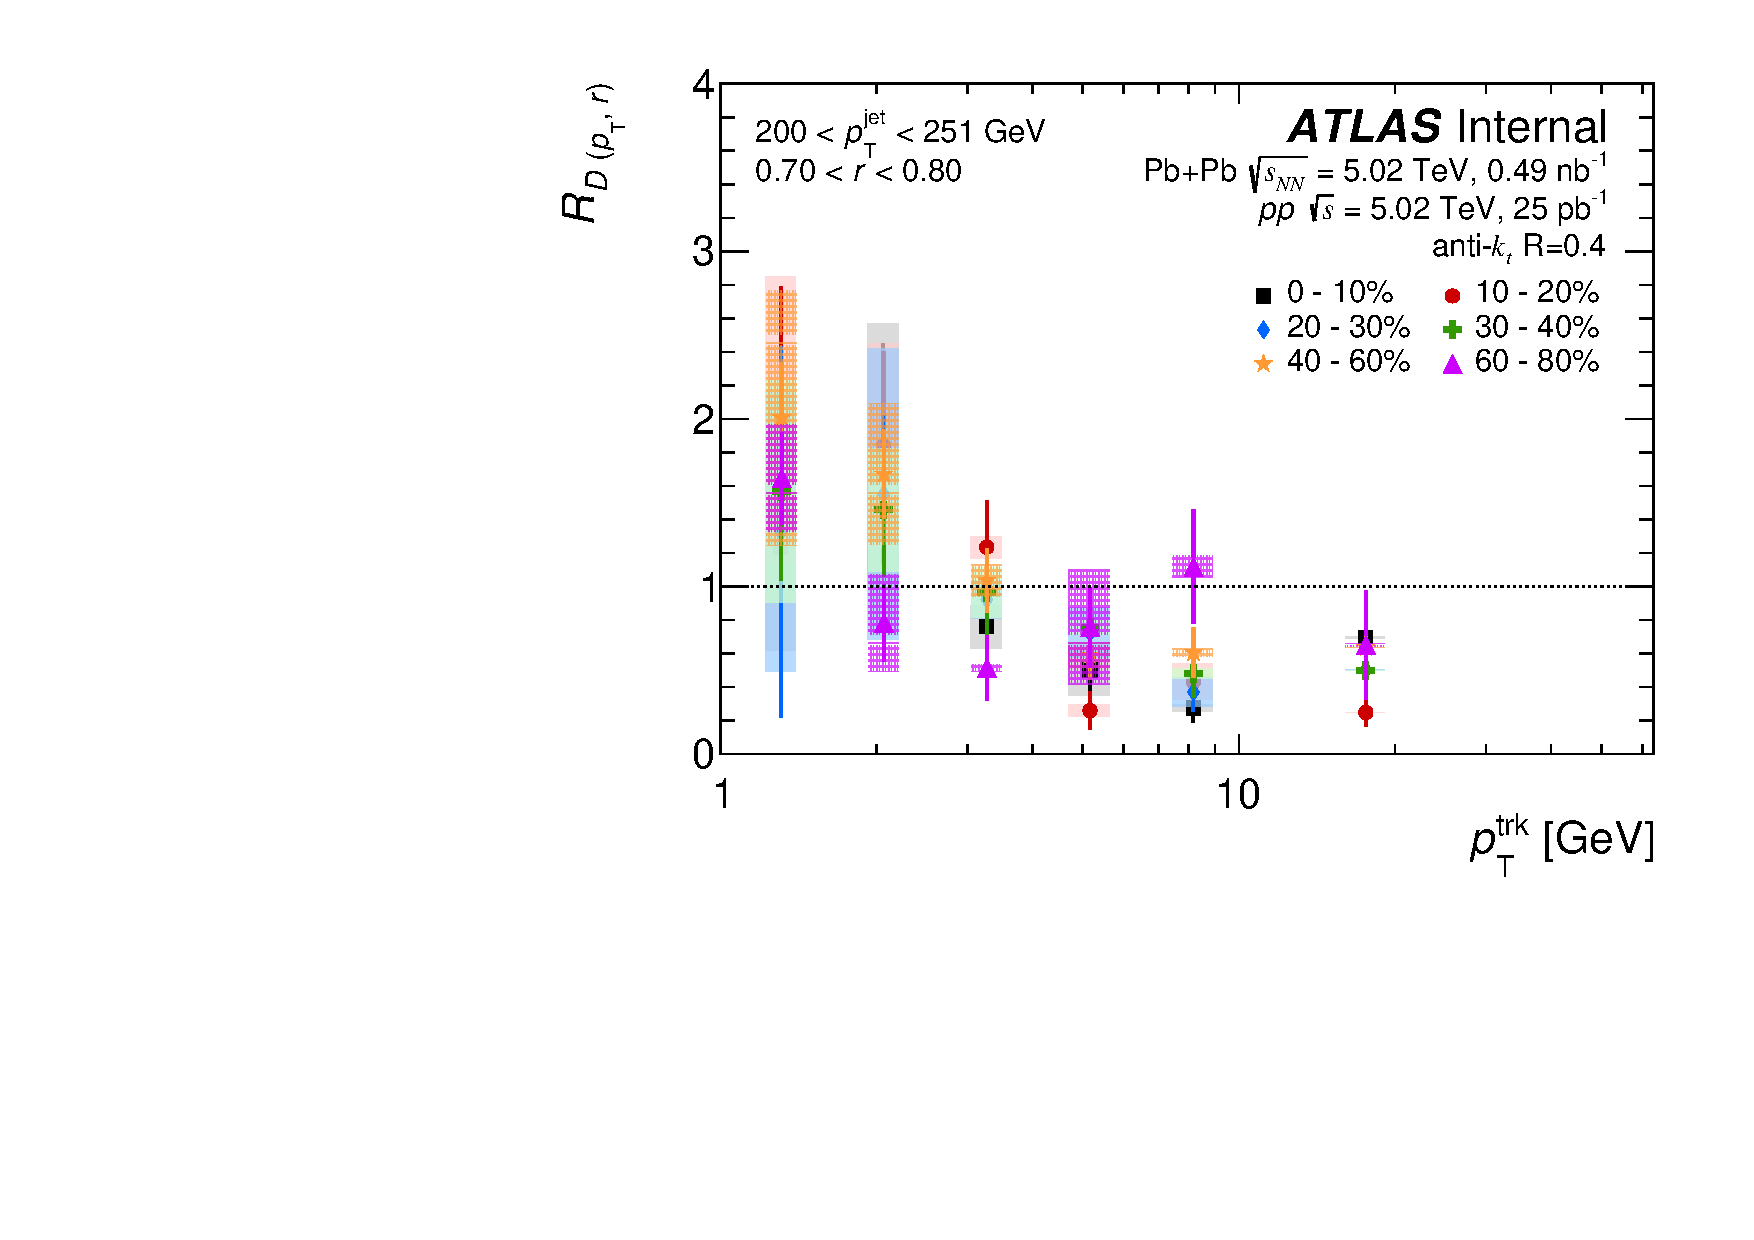
\includegraphics[width=0.5\textwidth]{results/xRDpT_final_ratio_dR_CONF_data_trkpT_jet9_dR10} \\
\end{tabular} }
   \caption{\RDptr\ for central \pbpb\ collisions as a function of \pt\ for $126 < \ptjet < 158$ GeV (left) and $200 < \ptjet < 251$ GeV (left) for three different distances from the jet axis: $0.00 < \rvar < 0.05$ (top), $0.15 < \rvar < 0.20$ (middle), $0.70 < \rvar < 0.80$ (bottom)}
      \label{fig:xrdptr}
\end{figure}




\FloatBarrier
